% ============================================================
%  Dobot CR5AS Manual
%  ------------------------------------------------------------
%  Expected folder structure (as described):
%      Desktop/Manual/manual.tex        <- this file
%      Desktop/Manual/Photos/*.png      <- all screenshots
%
%  Compile with pdflatex (run twice if the Table of Contents
%  or cross-references look out of date on the first pass).
%
%  Notes for you, Martina:
%   - I resolved the "CALLBACK" / "[LINK TO SECTION]" placeholders
%     into real LaTeX cross-references (\ref{...}), since that's
%     exactly what LaTeX's labelling system is for. Section
%     numbers will now update automatically if you reorder things.
%   - The "[PHOTO]" placeholder (IP selection screenshot in
%     "Connecting to the Dobot") doesn't have a filename yet in
%     your draft - I've left a clearly marked TODO figure block
%     for it, using a placeholder filename you'll need to swap in.
%   - Italian translation is NOT done here - this is a straight
%     LaTeX conversion of your current English text, since
%     translation was still an open checklist item.
% ============================================================

\documentclass[11pt,a4paper]{article}

% ---------- Encoding, fonts, symbols ----------
\usepackage[utf8]{inputenc}
\usepackage[T1]{fontenc}
\usepackage{textcomp}   % gives us \textdegree, \textpm, etc.
\usepackage[osf]{XCharter}   % warm, humanist serif - closest free match to Claude's UI font

% ---------- Page layout ----------
\usepackage[a4paper,margin=2.5cm]{geometry}
\usepackage{parskip}    % paragraph spacing instead of indentation
\usepackage{titlesec}

% ---------- Tables ----------
\usepackage{array}
\usepackage{longtable}
\usepackage{booktabs}
\usepackage{tabularx}

% ---------- Lists ----------
\usepackage{enumitem}

% ---------- Images ----------
\usepackage{graphicx}
\usepackage{float}   % lets us pin images exactly in place with [H], no drifting
\graphicspath{{Photos/}}   % lets us write 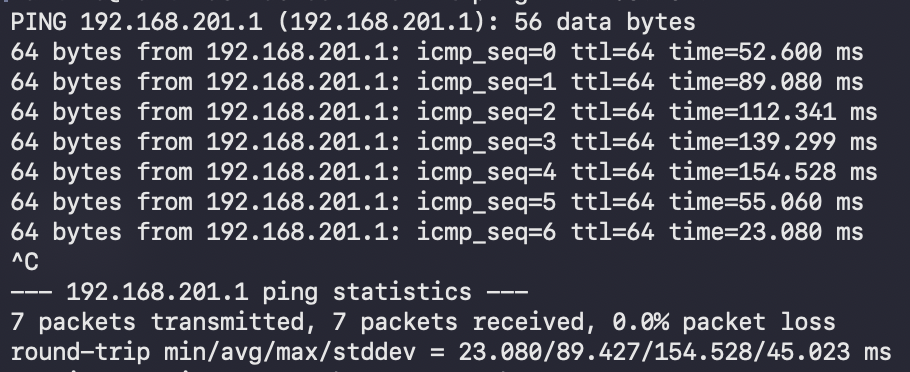
\includegraphics{1.png} instead of the full path

% ---------- Colors ----------
\usepackage{xcolor}
\definecolor{codepink}{RGB}{176,32,96}
\definecolor{codebg}{RGB}{245,245,245}

% ---------- Code blocks / inline code ----------
\usepackage{listings}
\lstdefinestyle{inline}{
    basicstyle=\ttfamily\small\color{codepink},
    breaklines=true,
    showstringspaces=false
}
\lstdefinestyle{block}{
    backgroundcolor=\color{codebg},
    basicstyle=\ttfamily\small,
    breaklines=true,
    frame=single,
    rulecolor=\color{gray!50},
    xleftmargin=2pt,
    xrightmargin=2pt,
    aboveskip=8pt,
    belowskip=8pt,
    showstringspaces=false
}
\lstset{style=block}

% Shorthand for inline code snippets, e.g. \code{EnableRobot()}
\newcommand{\code}[1]{\lstinline[style=inline]{#1}}

% ---------- Hyperlinks ----------
\usepackage[colorlinks=true, linkcolor=blue!50!black, urlcolor=blue!50!black, citecolor=black]{hyperref}

% ---------- Section spacing tweak ----------
\titlespacing*{\section}{0pt}{1.5\baselineskip}{0.8\baselineskip}
\titlespacing*{\subsection}{0pt}{1.2\baselineskip}{0.6\baselineskip}

\title{\textbf{Dobot CR5AS Manual}}
\author{Martina}
\date{}

\begin{document}

\maketitle
\tableofcontents
\newpage

% ============================================================
\section{Introduction}
\label{sec:introduction}
% ============================================================

I have had the opportunity to use the Dobot CR5AS robot arm at the association Asperastra in Trieste. I had some troubles finding out how to go past the basic features with the proprietary software, so I thought I collected what I learned in a file in order to help anyone who would like to learn to control it.

This manual includes information regarding the Dobot CR5AS robot arm with the DH Robotics PGC-140 gripper.

If you need any help or find any error, please feel free to reach out at \href{mailto:martinaanese05@gmail.com}{martinaanese05@gmail.com}.

Have fun!

% ============================================================
\section{Specs and data}
\label{sec:specs}
% ============================================================

\subsection{Specifics of CR5AS}
\label{sec:specs-cr5as}

\begin{longtable}{@{}p{5cm}p{9cm}@{}}
\toprule
\textbf{Spec} & \textbf{Value} \\
\midrule
\endhead
Payload & 5 kg \\ \midrule
Working radius & 900 mm \\ \midrule
Maximum reach & 1096 mm \\ \midrule
Repeatability & $\pm$0.02 mm \\ \midrule
Robot weight & 23 kg \\ \midrule
Max speed & 2 m/s, 223\textdegree/s per joint \\ \midrule
Collision detection & Present \\ \midrule
SafeSkin range & non-contact, 5--15 cm \\ \midrule
SafeSkin speed & 0.01s detection cycle, 0.1s e-stop execution \\ \midrule
SafeSkin material detection & conductive materials only: human body, metals, liquids \\ \midrule
SafeSkin joints & J4, J5, J6 \\ \midrule
Degrees of Freedom & 6 \\ \midrule
Power & 100--240V AC in, 48V DC / 20A max out \\ \midrule
Environmental constraints & 0--45\textdegree C, <95\% humidity no condensation, IP20 \\
\bottomrule
\end{longtable}

\bigskip
\noindent The default password and values for the following elements are:
\label{sec:passwords}

\begin{longtable}{@{}p{6cm}p{8cm}@{}}
\toprule
\textbf{Element} & \textbf{Value} \\
\midrule
\endhead
WiFi name & DobotCR5AS-4520-1795 \\ \midrule
WiFi password & 1234567890 \\ \midrule
IP address (Ethernet cable) & Specific to each machine \\ \midrule
IP address (WiFi connectivity) & Specific to each machine \\ \midrule
Administrator mode password & 888888 \\
\bottomrule
\end{longtable}

\subsection{Specifics of DH Robotics PGC-140-50}
\label{sec:specs-gripper}

\begin{longtable}{@{}p{5cm}p{9cm}@{}}
\toprule
\textbf{Spec} & \textbf{Value} \\
\midrule
\endhead
Gripping force & 40--140 N \\ \midrule
Stroke & 50 mm \\ \midrule
Payload & 3 kg \\ \midrule
Repeatability & $\pm$0.03 mm \\ \midrule
Min opening/closing time & 0.6 s \\ \midrule
Weight & 1 kg \\ \midrule
Rated voltage & 24 V DC $\pm$ 10\% \\ \midrule
Rated current & 0.4 A \\ \midrule
Peak current & 1 A \\ \midrule
Noise emission & < 50 dB \\ \midrule
Recommended environment & 0--40\textdegree C, under 85\% RH, IP67 \\ \midrule
Communication interface & Standard: Modbus RTU (RS485), Digital I/O --- Optional: TCP/IP, USB2.0, CAN2.0A, PROFINET, EtherCAT \\ \midrule
Flange mounting & ISO 9409-1-50-4-M6 standard flange \\
\bottomrule
\end{longtable}

\subsection{Connectivity}
\label{sec:connectivity}

The CR5AS can communicate with the outside world in two different ways:

\begin{itemize}[leftmargin=1.2cm]
    \item \textbf{TCP/UDP, Server or Client:} can be viewed like a phone call. A server is the one sitting by the phone, with a fixed number (IP address + port), waiting for someone to call. A client is the one who dials, it reaches out and starts the connection.

    With TCP/UDP, the CR5AS can be set up as either:
    \begin{itemize}
        \item \textbf{Server:} Robot waits with a fixed IP; your PC connects to it. Usually used in projects where there is one PC controlling one robot with custom scripts.
        \item \textbf{Client:} Robot initiates the connection out to another device. Often used in industry setups where a central PLC acts as the server and multiple robots connect to it.
    \end{itemize}

    \item \textbf{Modbus, Master or Slave:} Modbus is an older, stricter industrial protocol. The Master is always the one asking questions (``what's your current position?'', ``turn on output 3'') while the Slave only ever answers and can't initiate questions on its own.

    The CR5AS is always the Slave in Modbus, it can never be the Master.
\end{itemize}

\begin{longtable}{@{}p{7cm}p{7cm}@{}}
\toprule
\textbf{If you're\ldots} & \textbf{Use\ldots} \\
\midrule
\endhead
Writing custom control software (Python, C++, your own app) & TCP/IP, robot as Server \\ \midrule
Integrating with an existing PLC/SCADA industrial line & Modbus, other device as Master \\ \midrule
Building a distributed system with multiple robots reporting to one hub & TCP/IP, robot as Client \\
\bottomrule
\end{longtable}

A useful example is the Dashboard, which allows the Dobot to be programmable with scripts and using external, non-official tools. With the Dashboard, the Dobot acts as the Server and your script acts as the Client.

The Dashboard is a communication channel (over TCP/IP, on port 29999) that lets a developer send commands to the robot from a script instead of using default elements like a Pendant (physical command center, not always included with the Dobot) or the software DobotStudio Pro.

Before using the Dashboard, the robot must be in TCP mode, which is described in Section~\ref{sec:enabling-disabling-tcp}.

The Dobot can either be controlled by scripts in TCP mode or via DobotStudio Pro, which limits the use of third-party or personal elements but is easier to use.

% ============================================================
\section{Safety protocols}
\label{sec:safety}
% ============================================================

Here are some good safety protocols to use the Dobot safely:

\begin{itemize}[leftmargin=1.2cm]
    \item Always keep the emergency stop button within reach and easily accessible. The e-stop is a physical hardware cutoff: it disconnects power directly, meaning it overrides any code or command currently running, no exceptions. Because it's hardware-level, even a frozen script or a bug in your program can't stop the e-stop from working.
    \item Keep a clear working space around the robot at all times: no tools, cables, or fragile objects within its reach.
    \item Stay physically away from the robot's range of motion whenever it's powered on, even if it looks idle.
    \item Try to always keep SafeSkin active when working near the robot, especially during testing or development. SafeSkin only detects conductive material (skin, metal, liquids); it won't reliably sense non-conductive objects, so don't rely on it as your only safeguard.
    \item Test new scripts at reduced speed first, especially before running unfamiliar motion sequences.
    \item If anything behaves unexpectedly (unexpected motion, delayed response, strange sounds), hit the e-stop first, ask questions after.
\end{itemize}

% ============================================================
\section{Connecting to the Dobot}
\label{sec:connecting}
% ============================================================

\subsection{Using the DobotStudio Pro with a PC or tablet}
\label{sec:connecting-dobotstudio}

\begin{enumerate}[leftmargin=1.2cm]
    \item Turn the Dobot on, it'll take a couple of minutes to boot up and turn on its WiFi.
    \item Download the software from Dobot's Download Center (\url{https://www.Dobot-robots.com/service/download-center}) and start it.
    \item Connect to the WiFi (see name and password in Section~\ref{sec:passwords}). The Dobot creates its own personal WiFi that you can connect to (or use the Ethernet cable instead). Beware that when connected to its WiFi you will not have internet access.
    \item Follow the procedure in Section~\ref{sec:enabling-disabling-tcp} to turn TCP mode off. It only needs to be done the first time you connect after someone else could have turned TCP mode on. If you're the only one using it, you only need to redo this each time you switch modes, not every time you connect to the Dobot. If you skip this or forget, the software will tell you it can't control the robot because it's in TCP mode.
    \item In the software, press Connect, then select the robot with the correct IP.
\end{enumerate}

% TODO: you mentioned a [PHOTO] here in your draft showing the IP
% selection screen, but no filename was given yet. Once you have
% the screenshot, drop it in Photos/ and uncomment the block below,
% swapping in the real filename.
%
% \begin{figure}[H]
%     \centering
%     \includegraphics[width=0.8\textwidth]{connect_ip.png}
%     \caption{Selecting the robot by its IP address in DobotStudio Pro.}
% \end{figure}

Go to Section~\ref{sec:dobotstudio-guide} to learn about the main elements of the software.

\subsection{Using the Dashboard and TCP mode}
\label{sec:connecting-dashboard}

\begin{enumerate}[leftmargin=1.2cm]
    \item Turn the Dobot on, it'll take a couple of minutes to boot up and turn on its WiFi.
    \item Connect to the WiFi (see name and password in Section~\ref{sec:passwords}). The Dobot creates its own personal WiFi that you can connect to (or use the Ethernet cable instead). Beware that when connected to its WiFi you will not have internet access.
    \item Follow the procedure in Section~\ref{sec:enabling-disabling-tcp} to turn TCP mode on. It only needs to be done the first time you connect after someone else could have turned TCP mode off. If you're the only one using it, you only need to redo this each time you switch modes, not every time you connect to the Dobot. If you skip this or forget, you won't be able to program the Dobot freely.
\end{enumerate}

Go to Section~\ref{sec:python-programming} to learn about TCP programming.

\subsection{Enabling/Disabling TCP}
\label{sec:enabling-disabling-tcp}

I have added a video of the procedure to disable TCP (enabling it follows the same structure) in the repository this manual is attached to.

You need to enable TCP if you want to program it with custom Python scripts, and turn it off if you'd like to program it with the DobotStudio Pro software.

\subsubsection*{Enabling TCP}

\begin{enumerate}[leftmargin=1.2cm]

\item Turn on the Dobot, wait for it to boot completely and connect to its WiFi. Open the terminal.

The following code blocks include the example IP \code{192.168.201.1} and you will have to swap it out with your Dobot's IP.

For both Mac and Windows users:

\item Check the robot's connection:
\begin{lstlisting}[style=block,language=bash]
ping 192.168.201.1
\end{lstlisting}

On Mac, after a while you have to interrupt it with Control+C.

If run correctly, you'll get something like:

\begin{figure}[H]
    \centering
    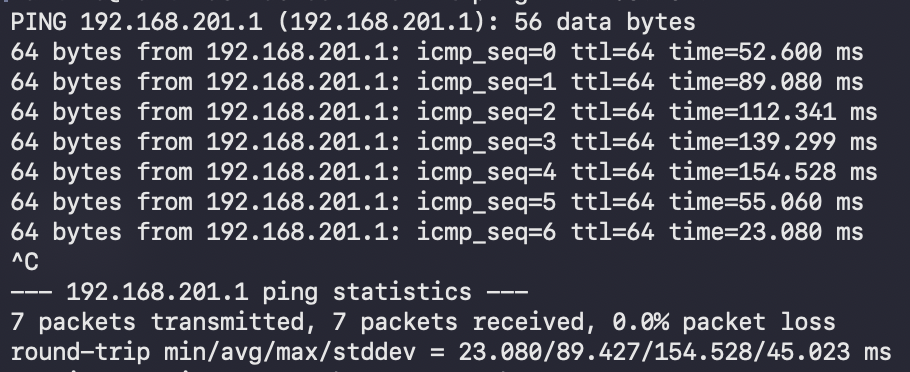
\includegraphics[width=0.8\textwidth]{1.png}
    \caption{Expected output of a successful \texttt{ping} to the robot.}
\end{figure}

If the packet loss is close to 0\%, you can continue. Otherwise, retry the ping or check that you are correctly connected to the Dobot's WiFi.

\item Connect via SSH:
\begin{lstlisting}[style=block,language=bash]
ssh root@192.168.201.1
\end{lstlisting}
This step may ask for a password, it's usually ``dobot''.

\item Backup the current settings:
\begin{lstlisting}[style=block,language=bash]
cp /dobot/userdata/project/settings/function/remoteControl.json /dobot/userdata/project/settings/function/remoteControl.json.bak
\end{lstlisting}

\item Set TCP mode:
\begin{lstlisting}[style=block,language=bash]
echo '{"mode":"tcp"}' > /dobot/userdata/project/settings/function/remoteControl.json
echo '{"mode":"tcp"}' > /dobot/userdata/user_project/settings/function/remoteControl.json
\end{lstlisting}

\item Enable the remote switch:
\begin{lstlisting}[style=block,language=bash]
echo '{"value": true}' > /dobot/userdata/project/settings/function/remoteSwitch.json
echo '{"value": true}' > /dobot/userdata/user_project/settings/function/remoteSwitch.json
\end{lstlisting}

\item Reboot:
\begin{lstlisting}[style=block,language=bash]
reboot
\end{lstlisting}

\item Then turn the Dobot off by pressing and holding the on/off button for 4 seconds, then wait for 30s and turn it back on by pressing the on/off button.

\end{enumerate}

\subsubsection*{Disabling TCP mode}

\begin{enumerate}[leftmargin=1.2cm]

\item Turn on the Dobot, wait for it to boot completely and connect to its WiFi. Open the terminal.

The following code blocks include the example IP \code{192.168.201.1} and you will have to swap it out with your Dobot's IP.

For both Mac and Windows users:

\item Check the robot's connection:
\begin{lstlisting}[style=block,language=bash]
ping 192.168.201.1
\end{lstlisting}

On Mac, after a while you have to interrupt it with Control+C.

If run correctly, you'll get something like:

\begin{figure}[H]
    \centering
    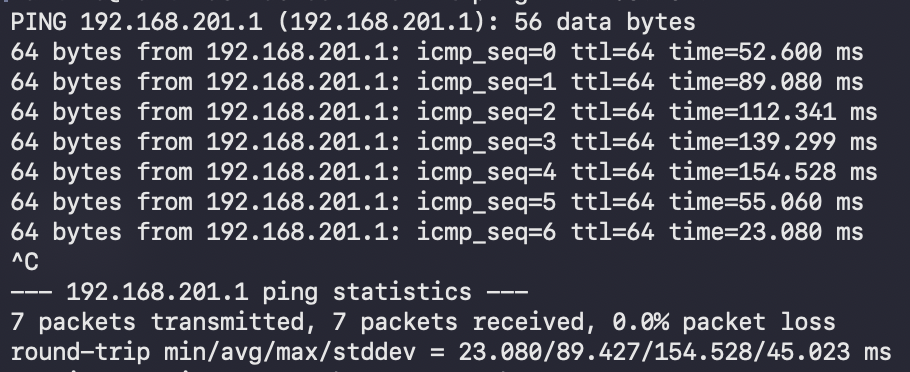
\includegraphics[width=0.8\textwidth]{2.png}
    \caption{Expected output of a successful \texttt{ping} to the robot.}
\end{figure}

If the packet loss is close to 0\%, you can continue. Otherwise, retry the ping or check that you are correctly connected to the Dobot's WiFi.

\item Connect via SSH:
\begin{lstlisting}[style=block,language=bash]
ssh root@192.168.201.1
\end{lstlisting}
This step may ask for a password, it's usually ``dobot''.

\item Backup the current settings:
\begin{lstlisting}[style=block,language=bash]
cp /dobot/userdata/project/settings/function/remoteControl.json /dobot/userdata/project/settings/function/remoteControl.json.bak
\end{lstlisting}

\item Set TP mode:
\begin{lstlisting}[style=block,language=bash]
echo '{"mode":"tp"}' > /dobot/userdata/project/settings/function/remoteControl.json
echo '{"mode":"tp"}' > /dobot/userdata/user_project/settings/function/remoteControl.json
\end{lstlisting}

\item Disable the remote switch:
\begin{lstlisting}[style=block,language=bash]
echo '{"value": false}' > /dobot/userdata/project/settings/function/remoteSwitch.json
echo '{"value": false}' > /dobot/userdata/user_project/settings/function/remoteSwitch.json
\end{lstlisting}

\item Reboot:
\begin{lstlisting}[style=block,language=bash]
reboot
\end{lstlisting}

\item Then turn the Dobot off by pressing and holding the on/off button for 4 seconds, then wait for 30s and turn it back on by pressing the on/off button.

\end{enumerate}

% ============================================================
\section{How to use DobotStudio Pro}
\label{sec:dobotstudio-guide}
% ============================================================

DobotStudio Pro is the original software to control and program any Dobot robotic arm.

Following is a brief explanation of the main features of the software, but I recommend taking a look at the file called ``DobotStudio Pro User Guide (CR\&Nova) V2.8.0'', which you can download at \url{https://www.Dobot-robots.com/service/download-center}, or taking a look at the site \url{https://docs.trossenrobotics.com/Dobot_cr_cobots_docs/Dobotstudiopro/programming.html}, where they go deeper into it.

\begin{itemize}[leftmargin=1.2cm]

\item This is the page the software opens on. With ``Connect'', you'll be able to select your Dobot by its IP and connect to it. Make sure you're connected to the Dobot's WiFi.

\begin{figure}[H]
    \centering
    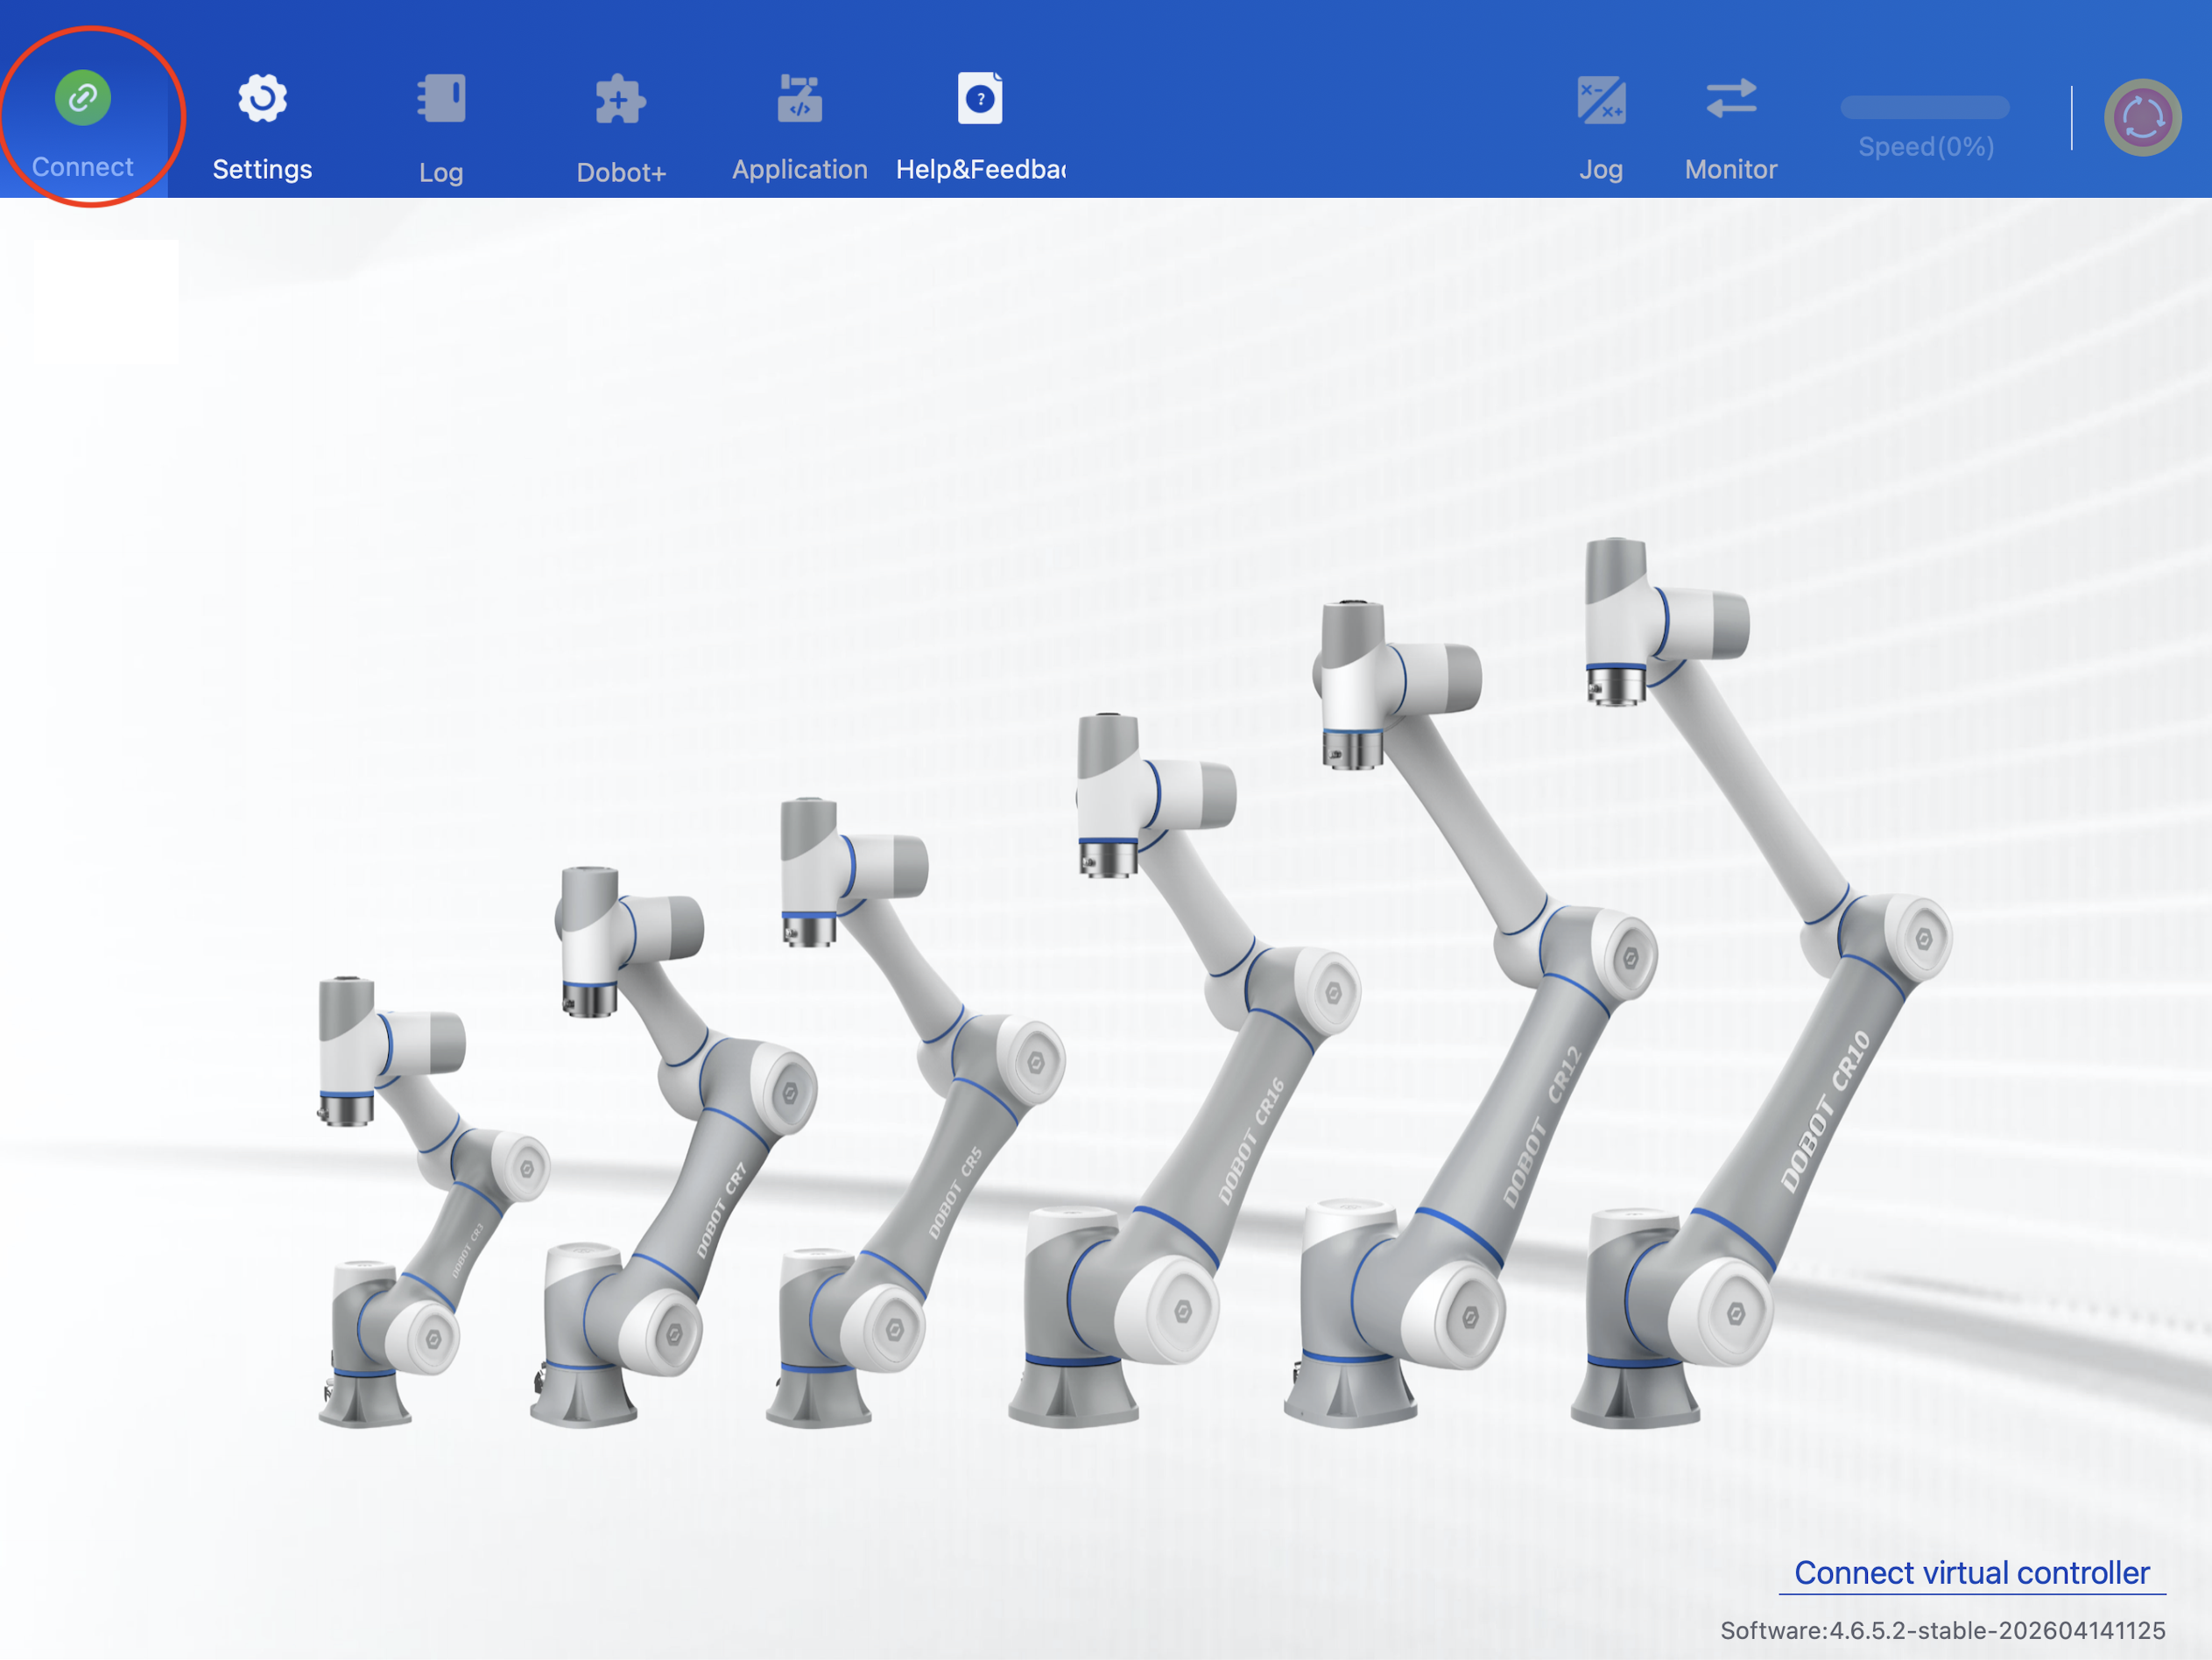
\includegraphics[width=0.9\textwidth]{3.png}
\end{figure}

\item By pressing ``Enable'', you're enabling the Dobot to be controlled. Note that on the right side of the screen you're able to see the Dobot's position at any time and, if SafeSkin is on, to see if parts of it detect a close object.

The color of the little Dobot icon in the top left corner is indicative of its status: blue means disabled, green means enabled and working correctly, yellow means there is a non-threatening error (such as a collision with the SafeSkin), and red means a threatening error.

\begin{figure}[H]
    \centering
    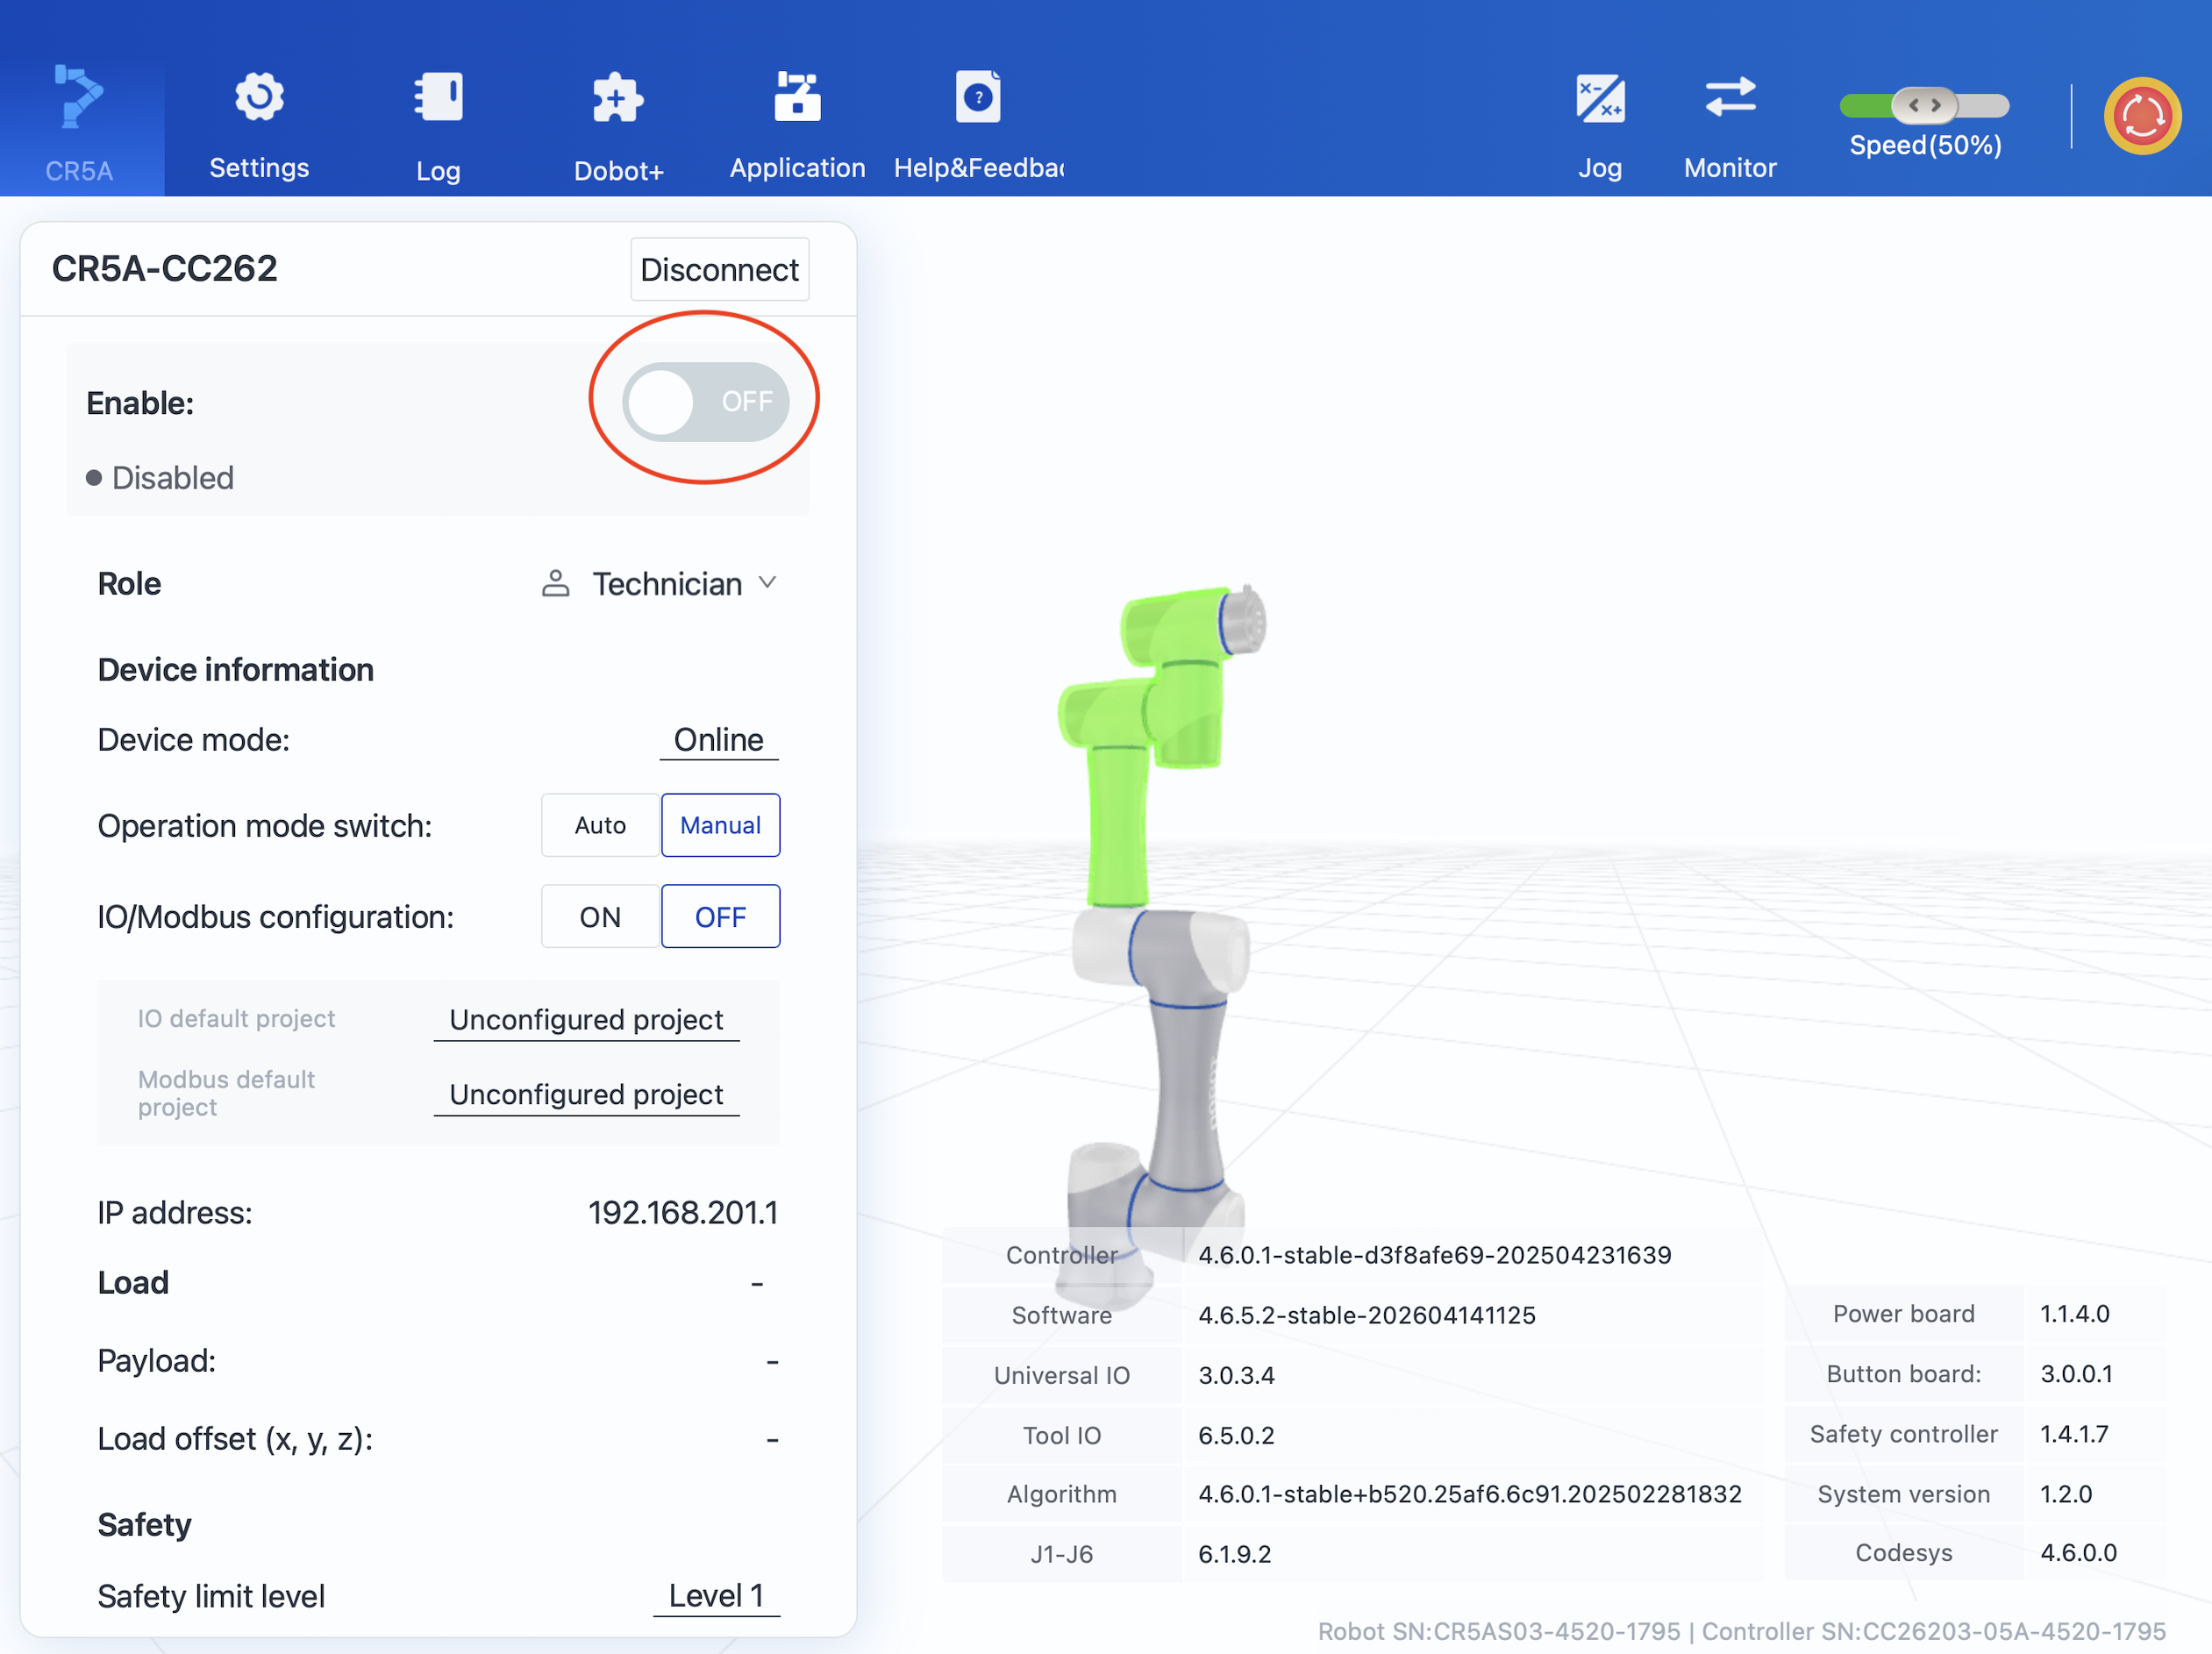
\includegraphics[width=0.9\textwidth]{4.png}
\end{figure}

\item Once you press Enable, the Dobot will perform a Load examination. If the numbers are correct, confirm Enable.

\begin{figure}[H]
    \centering
    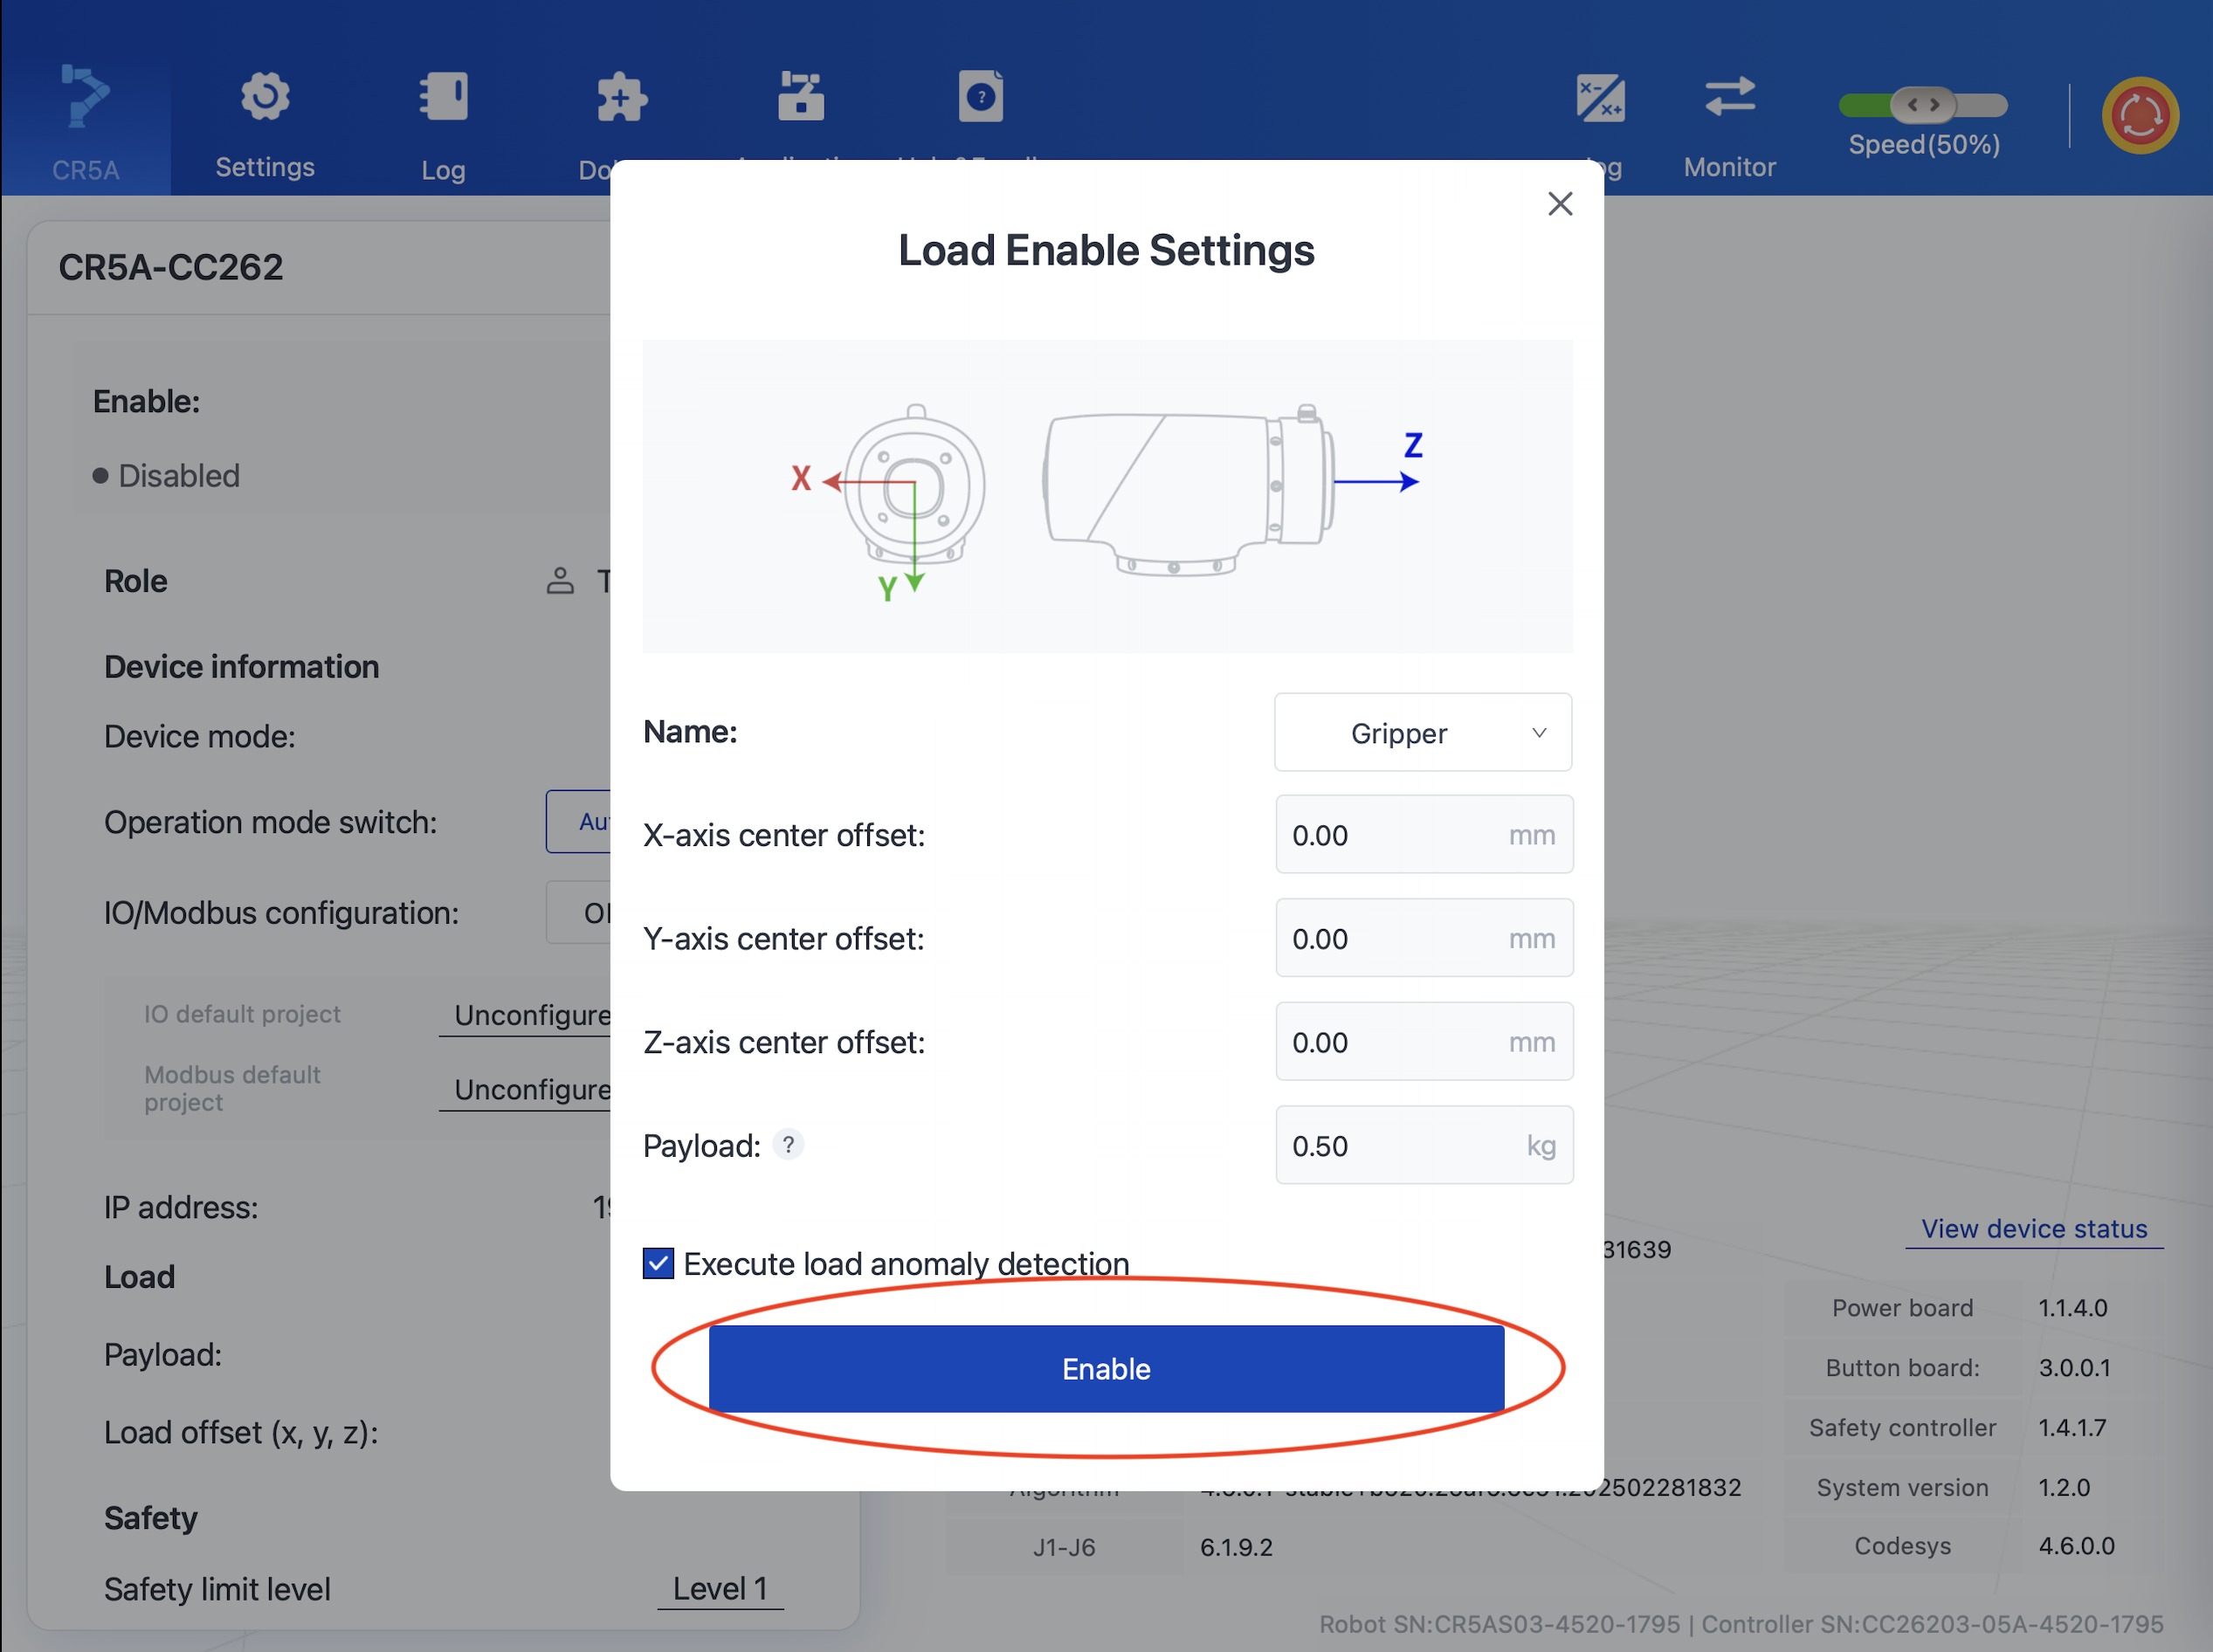
\includegraphics[width=0.9\textwidth]{5.png}
\end{figure}

\item By selecting ``Jog'' you are able to move the Dobot one joint at a time. This option also contains ``Target Pose'', with which you'll be able to gradually move the Dobot to some predefined positions like Safe Home and Pack Pose.

\begin{figure}[H]
    \centering
    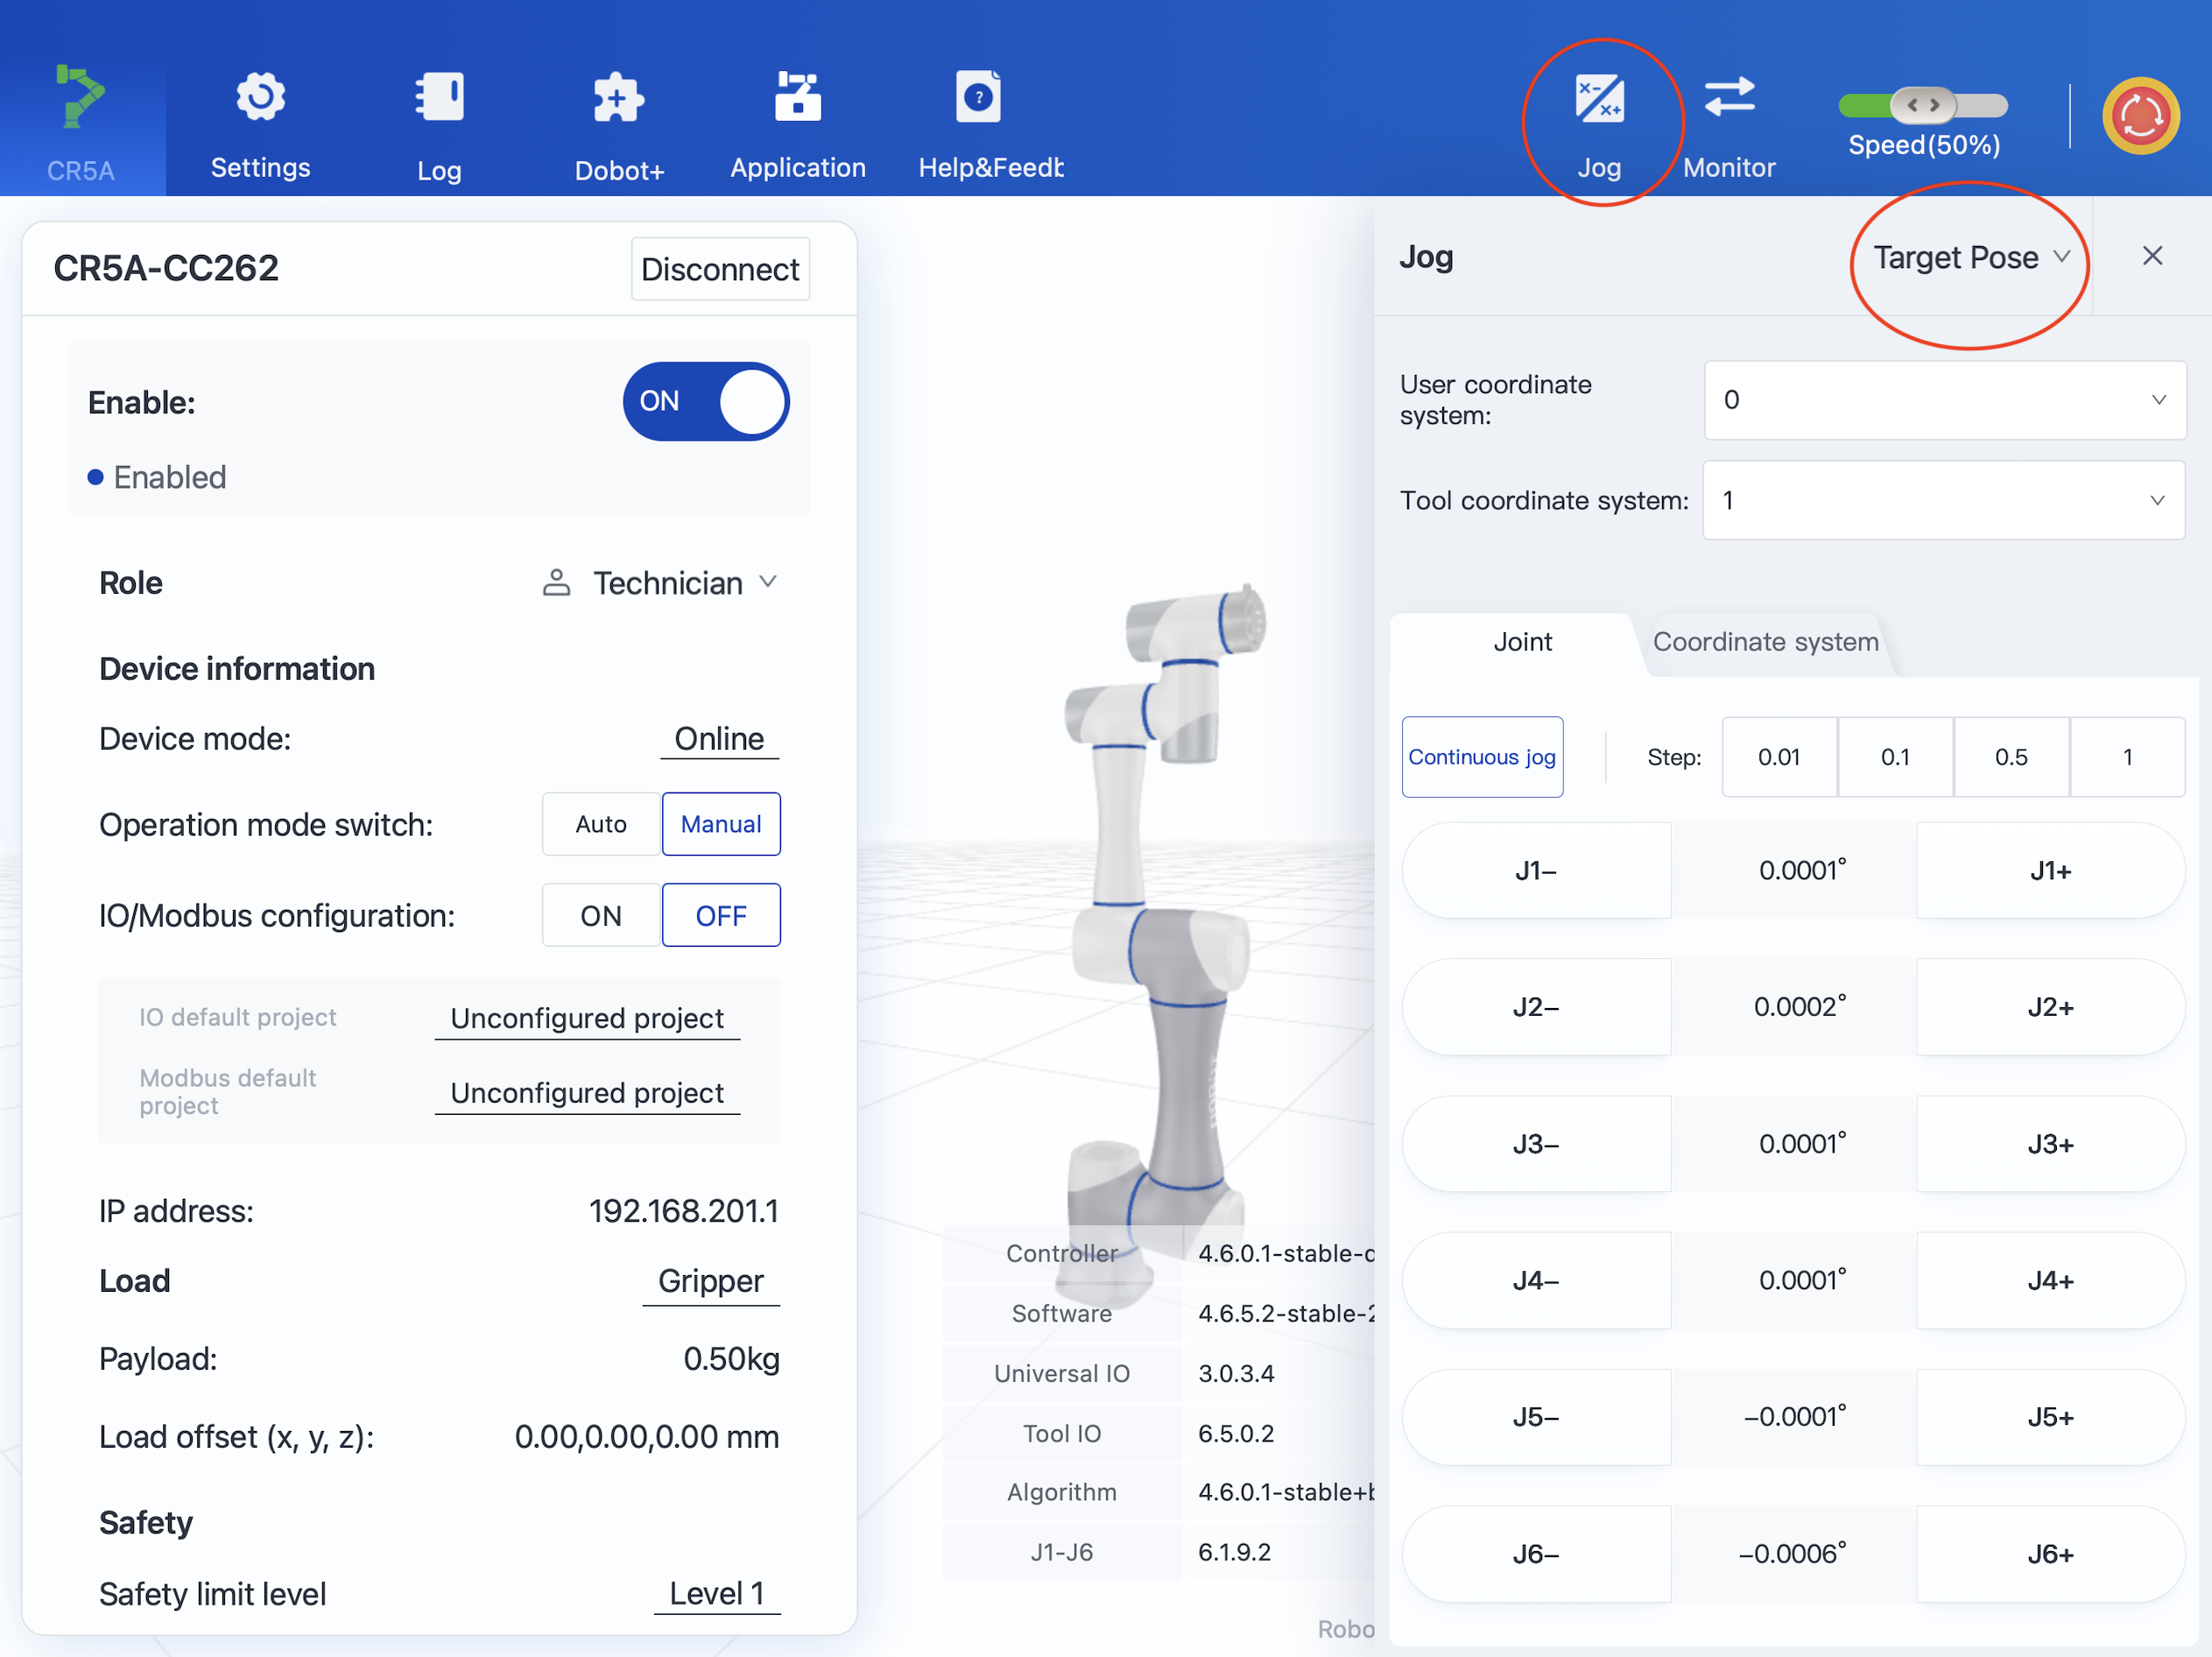
\includegraphics[width=0.9\textwidth]{6.png}
\end{figure}

\begin{figure}[H]
    \centering
    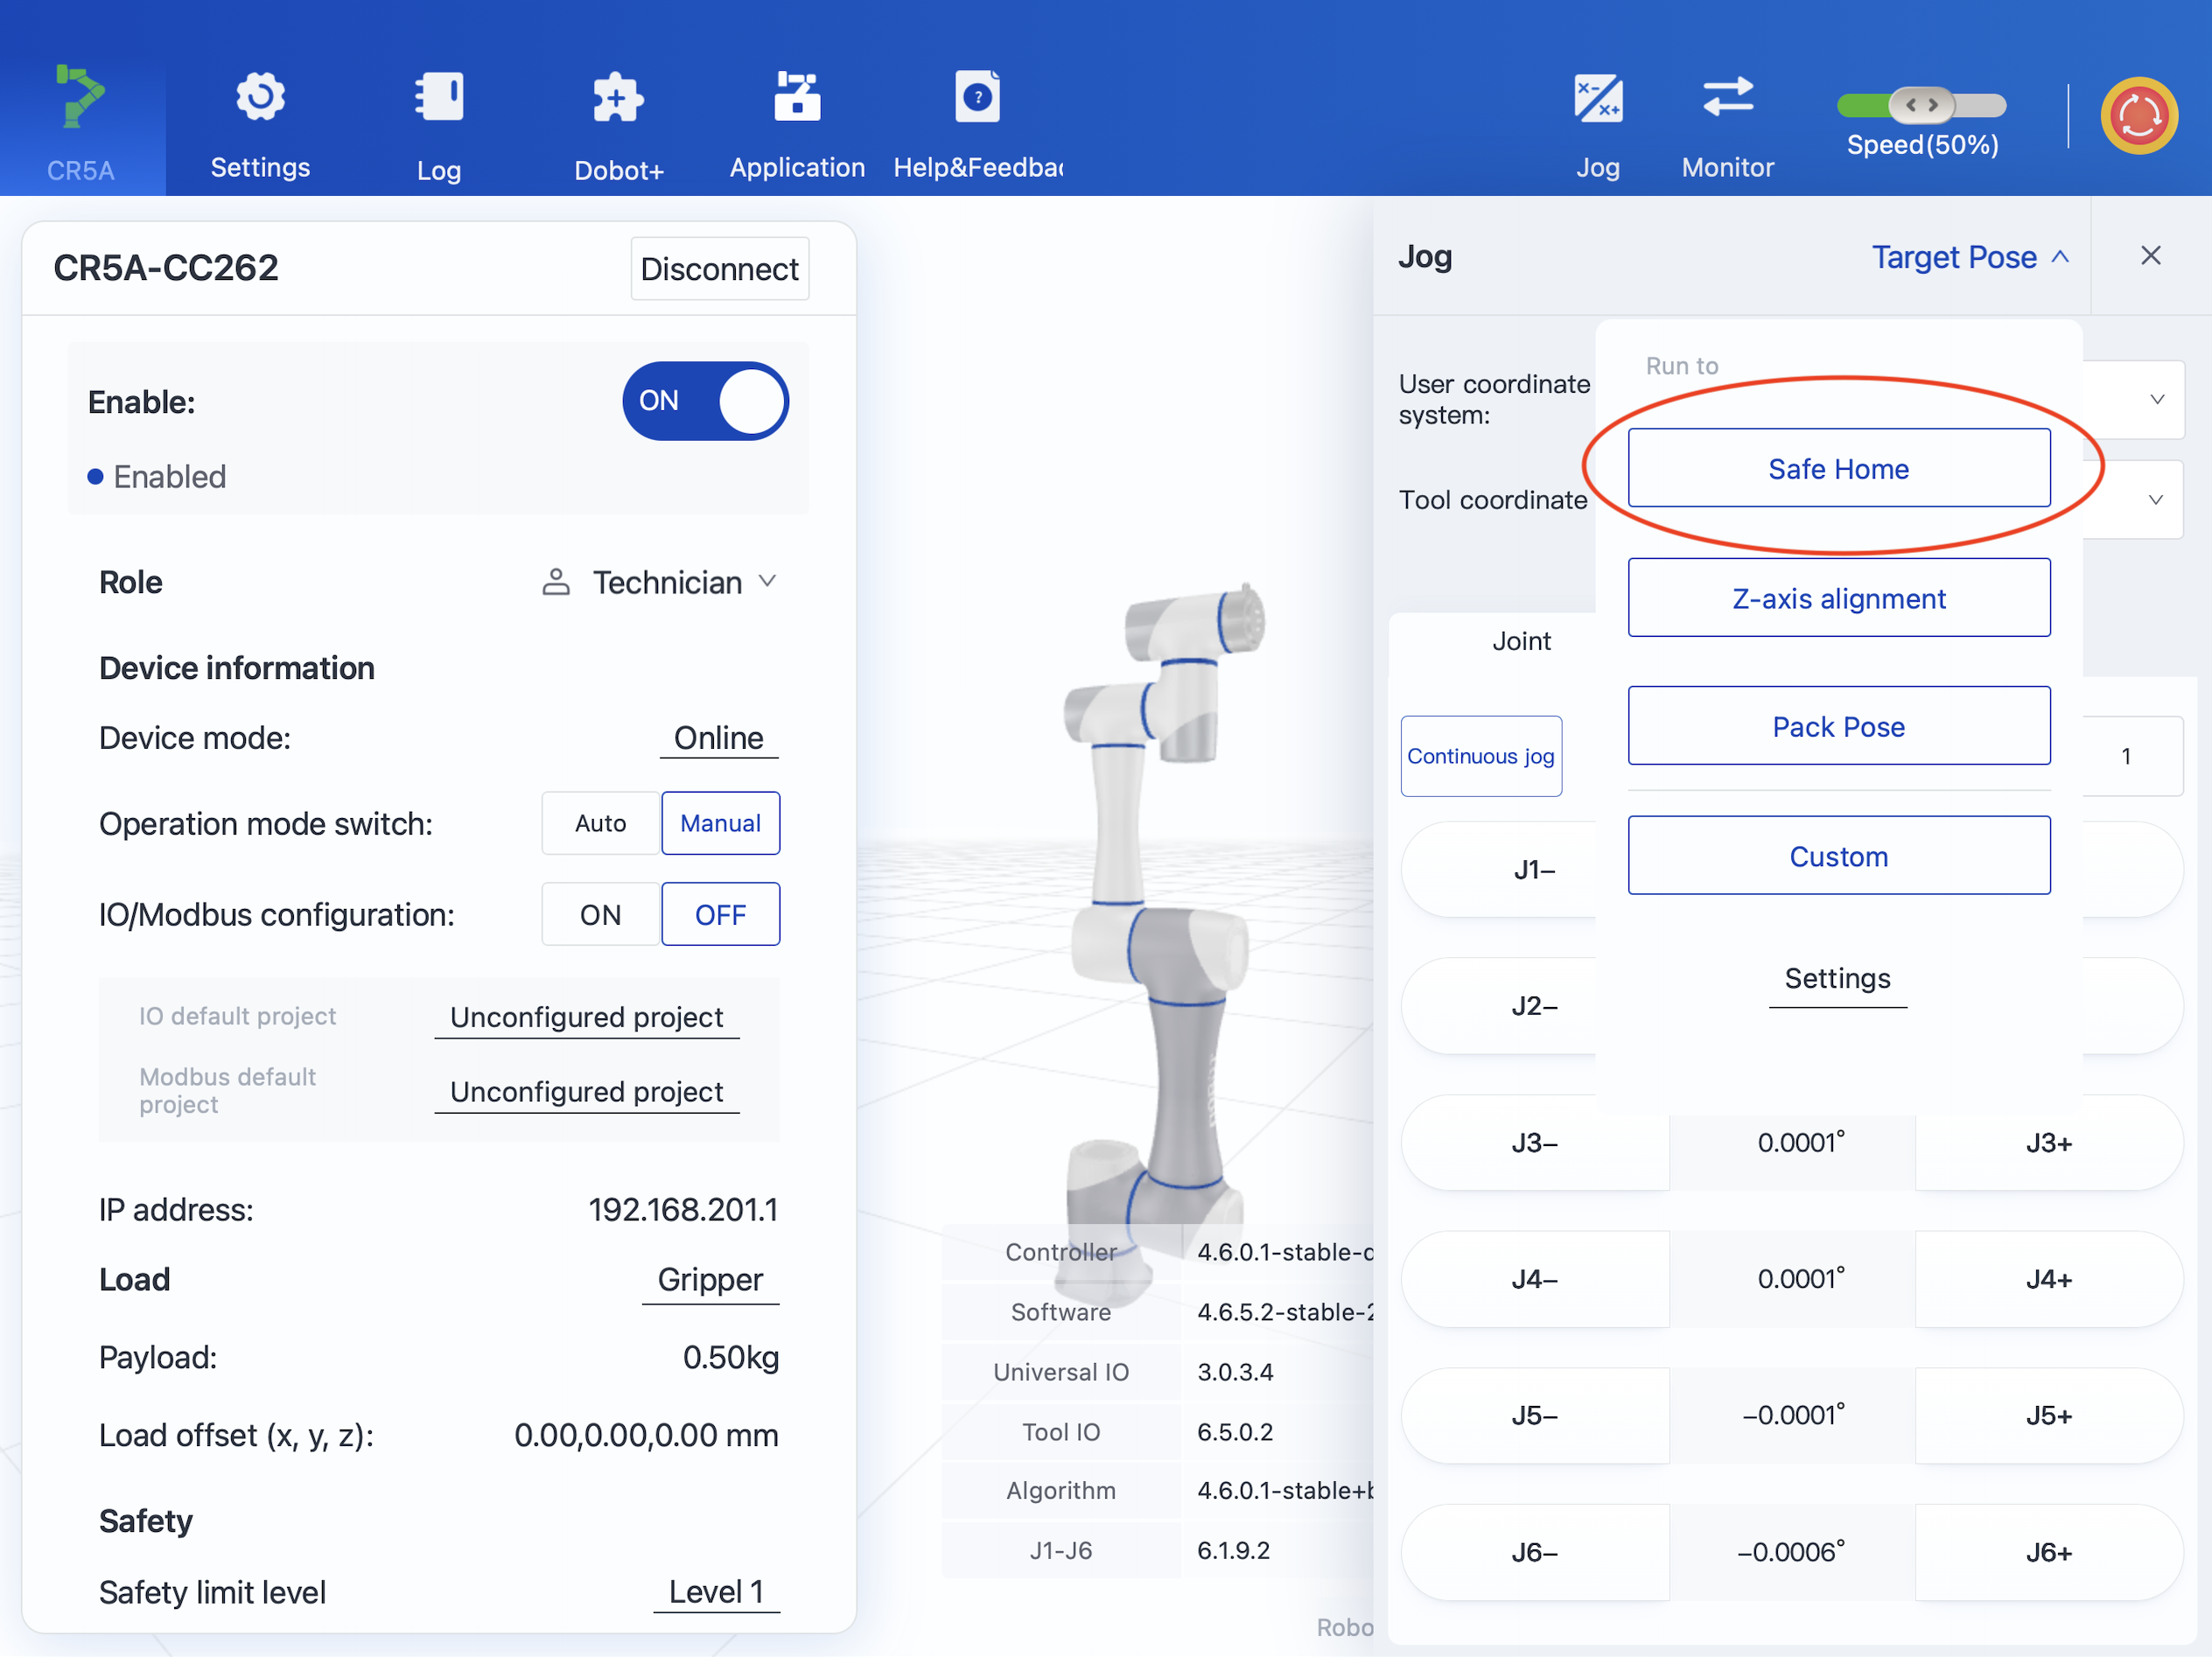
\includegraphics[width=0.9\textwidth]{7.png}
\end{figure}

\item By selecting ``Monitor'' you'll be able to dive into more functions related to Input/Output.

\begin{figure}[H]
    \centering
    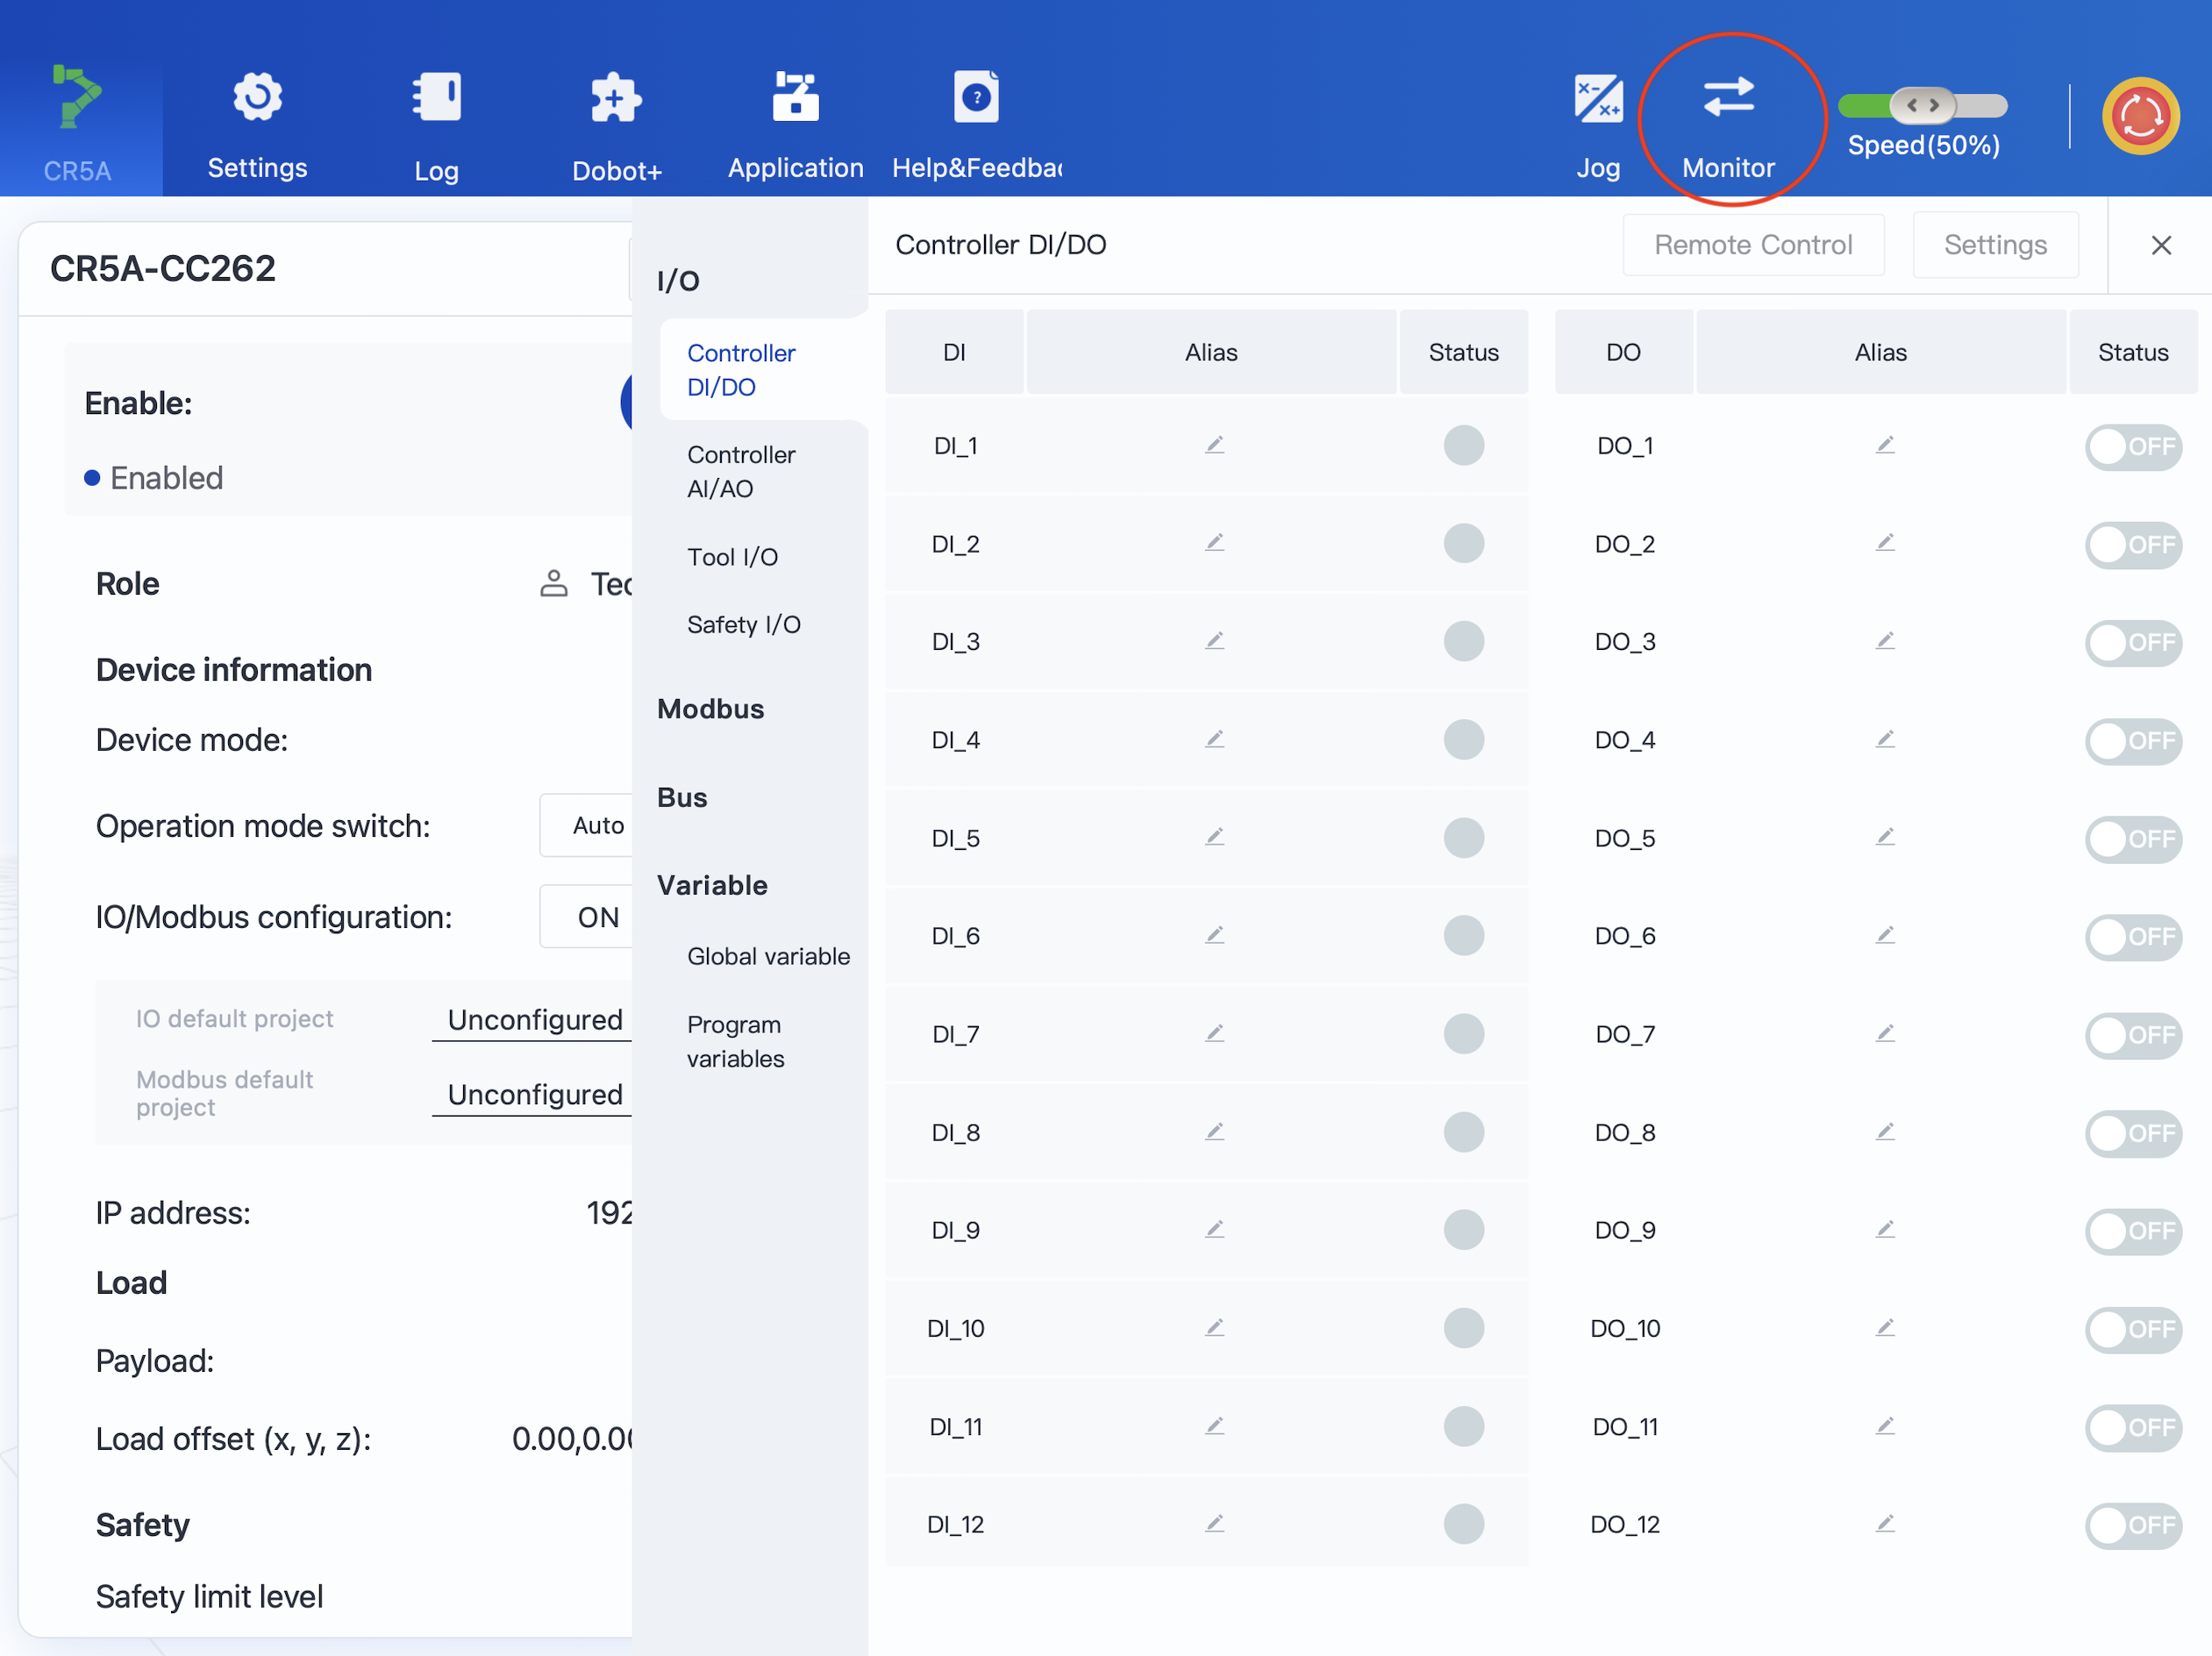
\includegraphics[width=0.9\textwidth]{8.png}
\end{figure}

\item This is the Settings panel, which allows you to tweak the Dobot. An important setting to note is that by going into ``Communications'' you'll be able to view and edit the Dobot's IP address.

\begin{figure}[H]
    \centering
    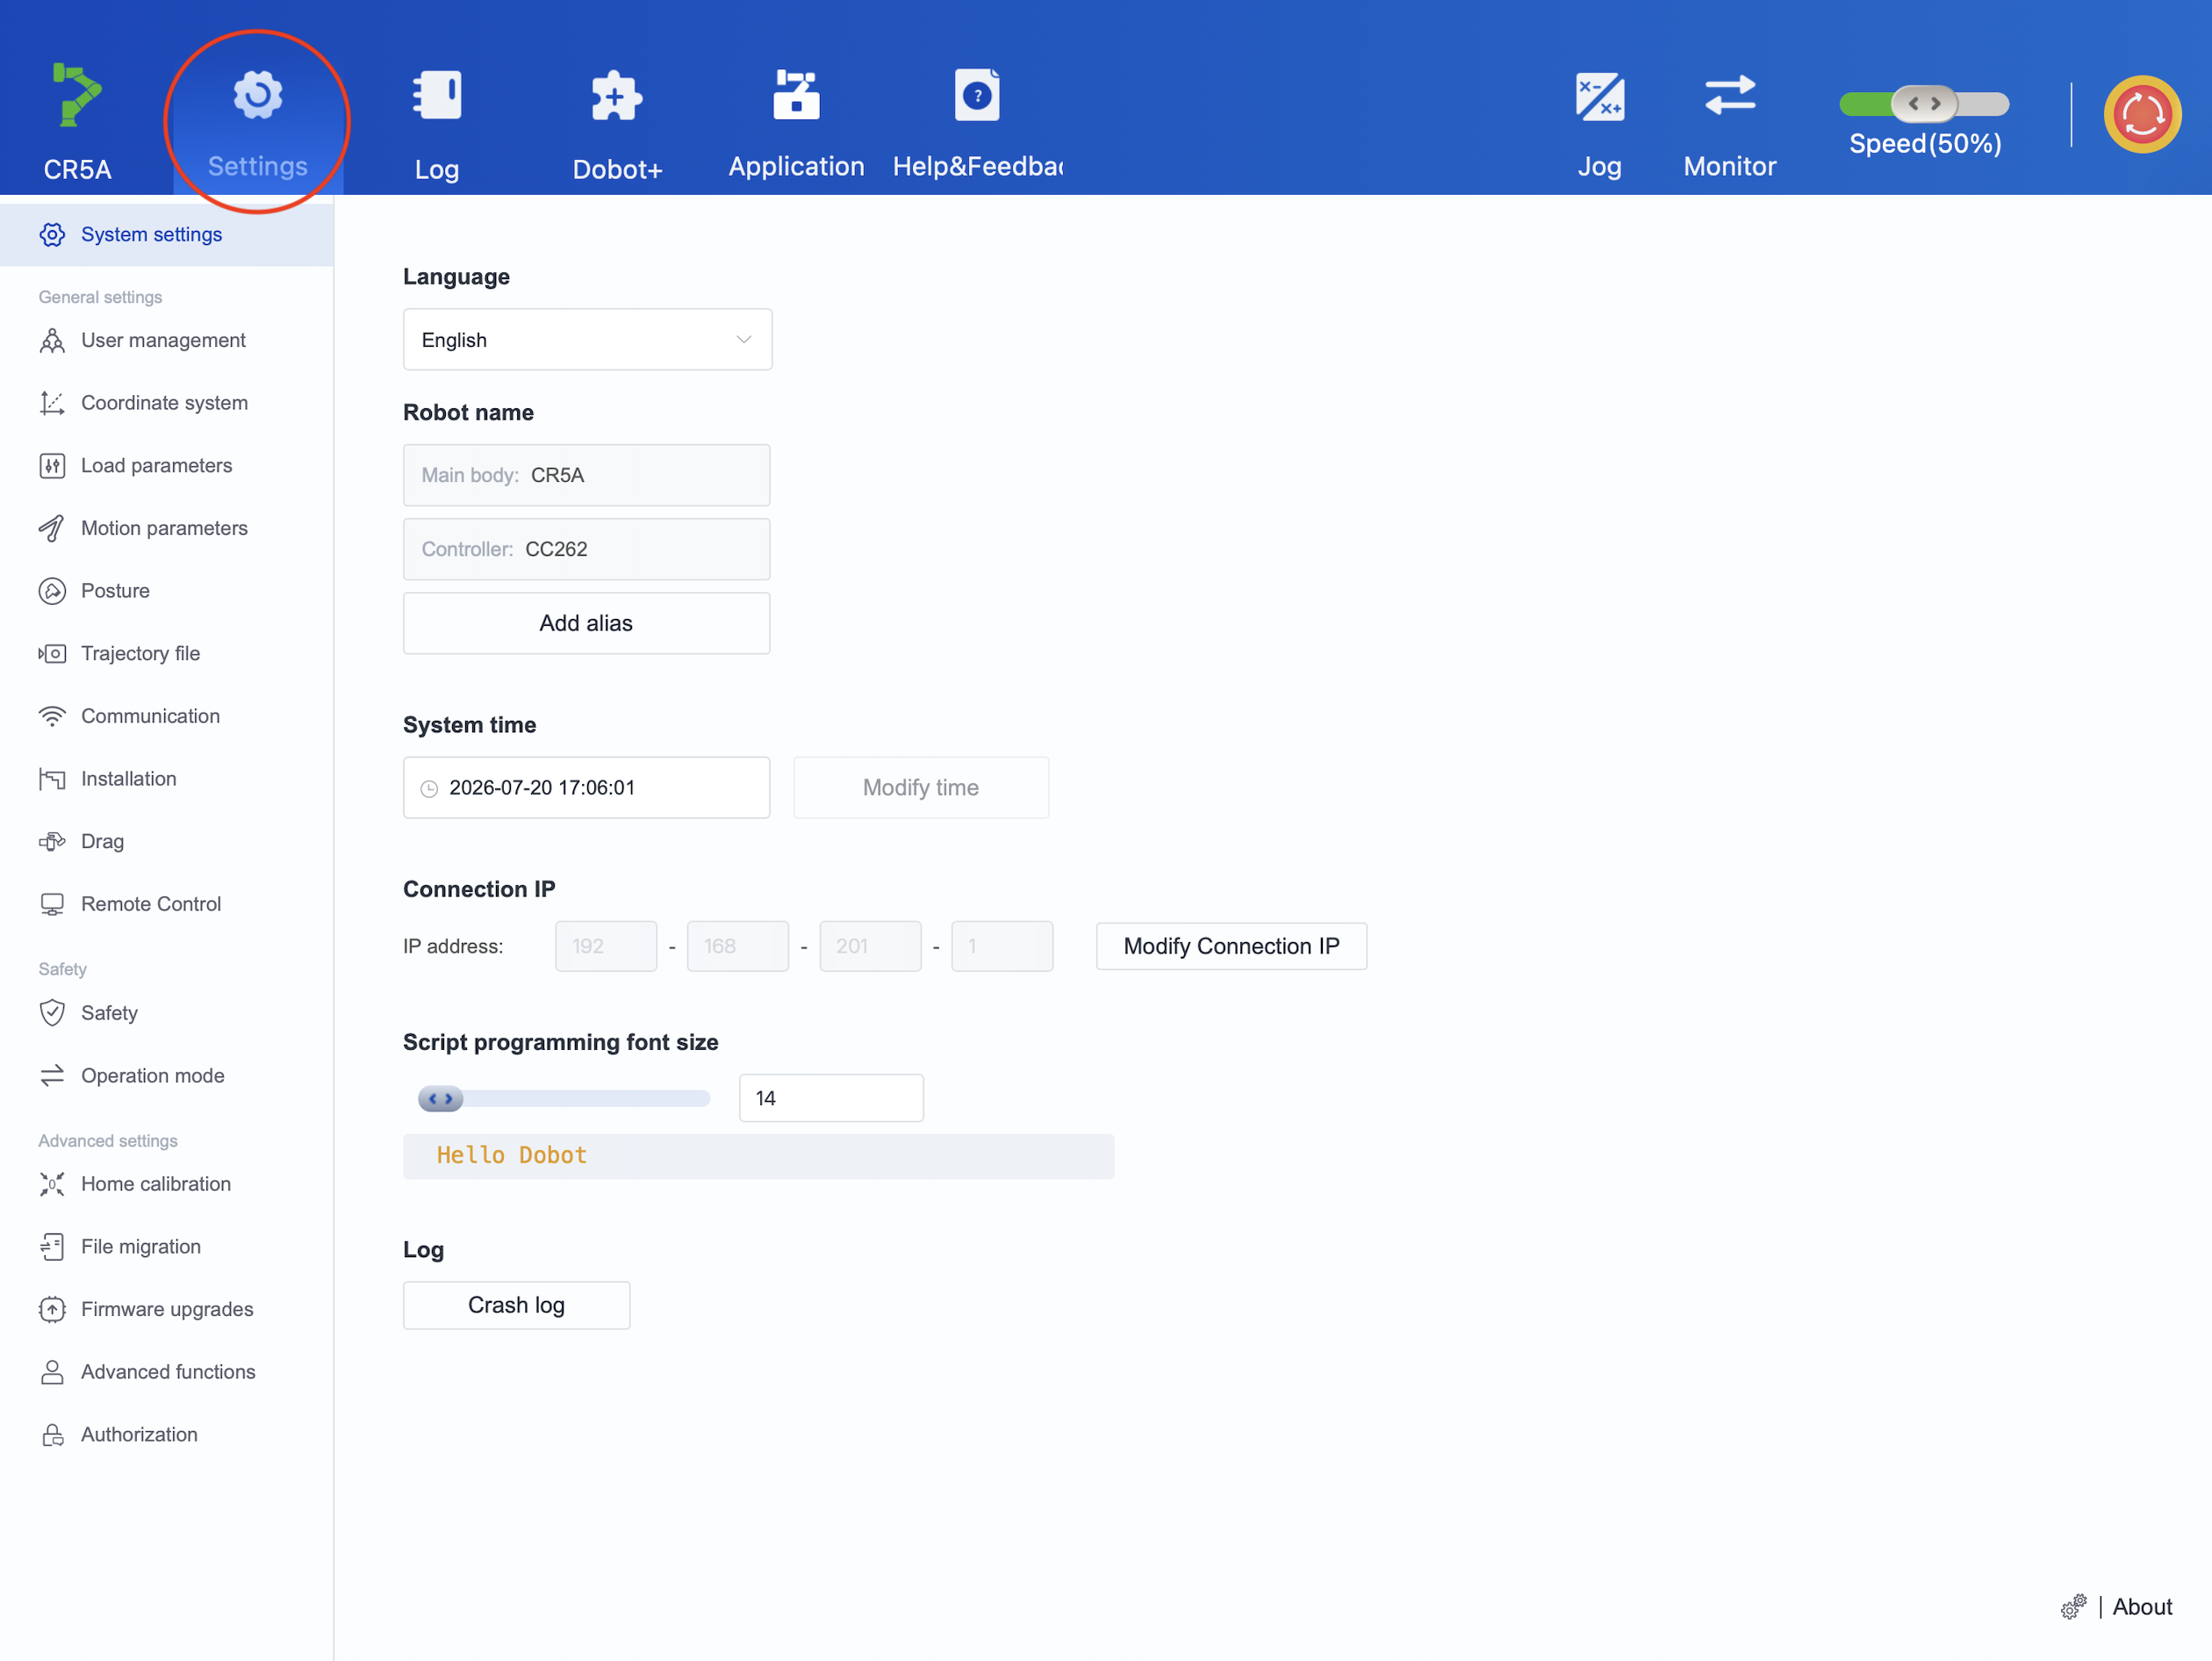
\includegraphics[width=0.9\textwidth]{9.png}
\end{figure}

\begin{figure}[H]
    \centering
    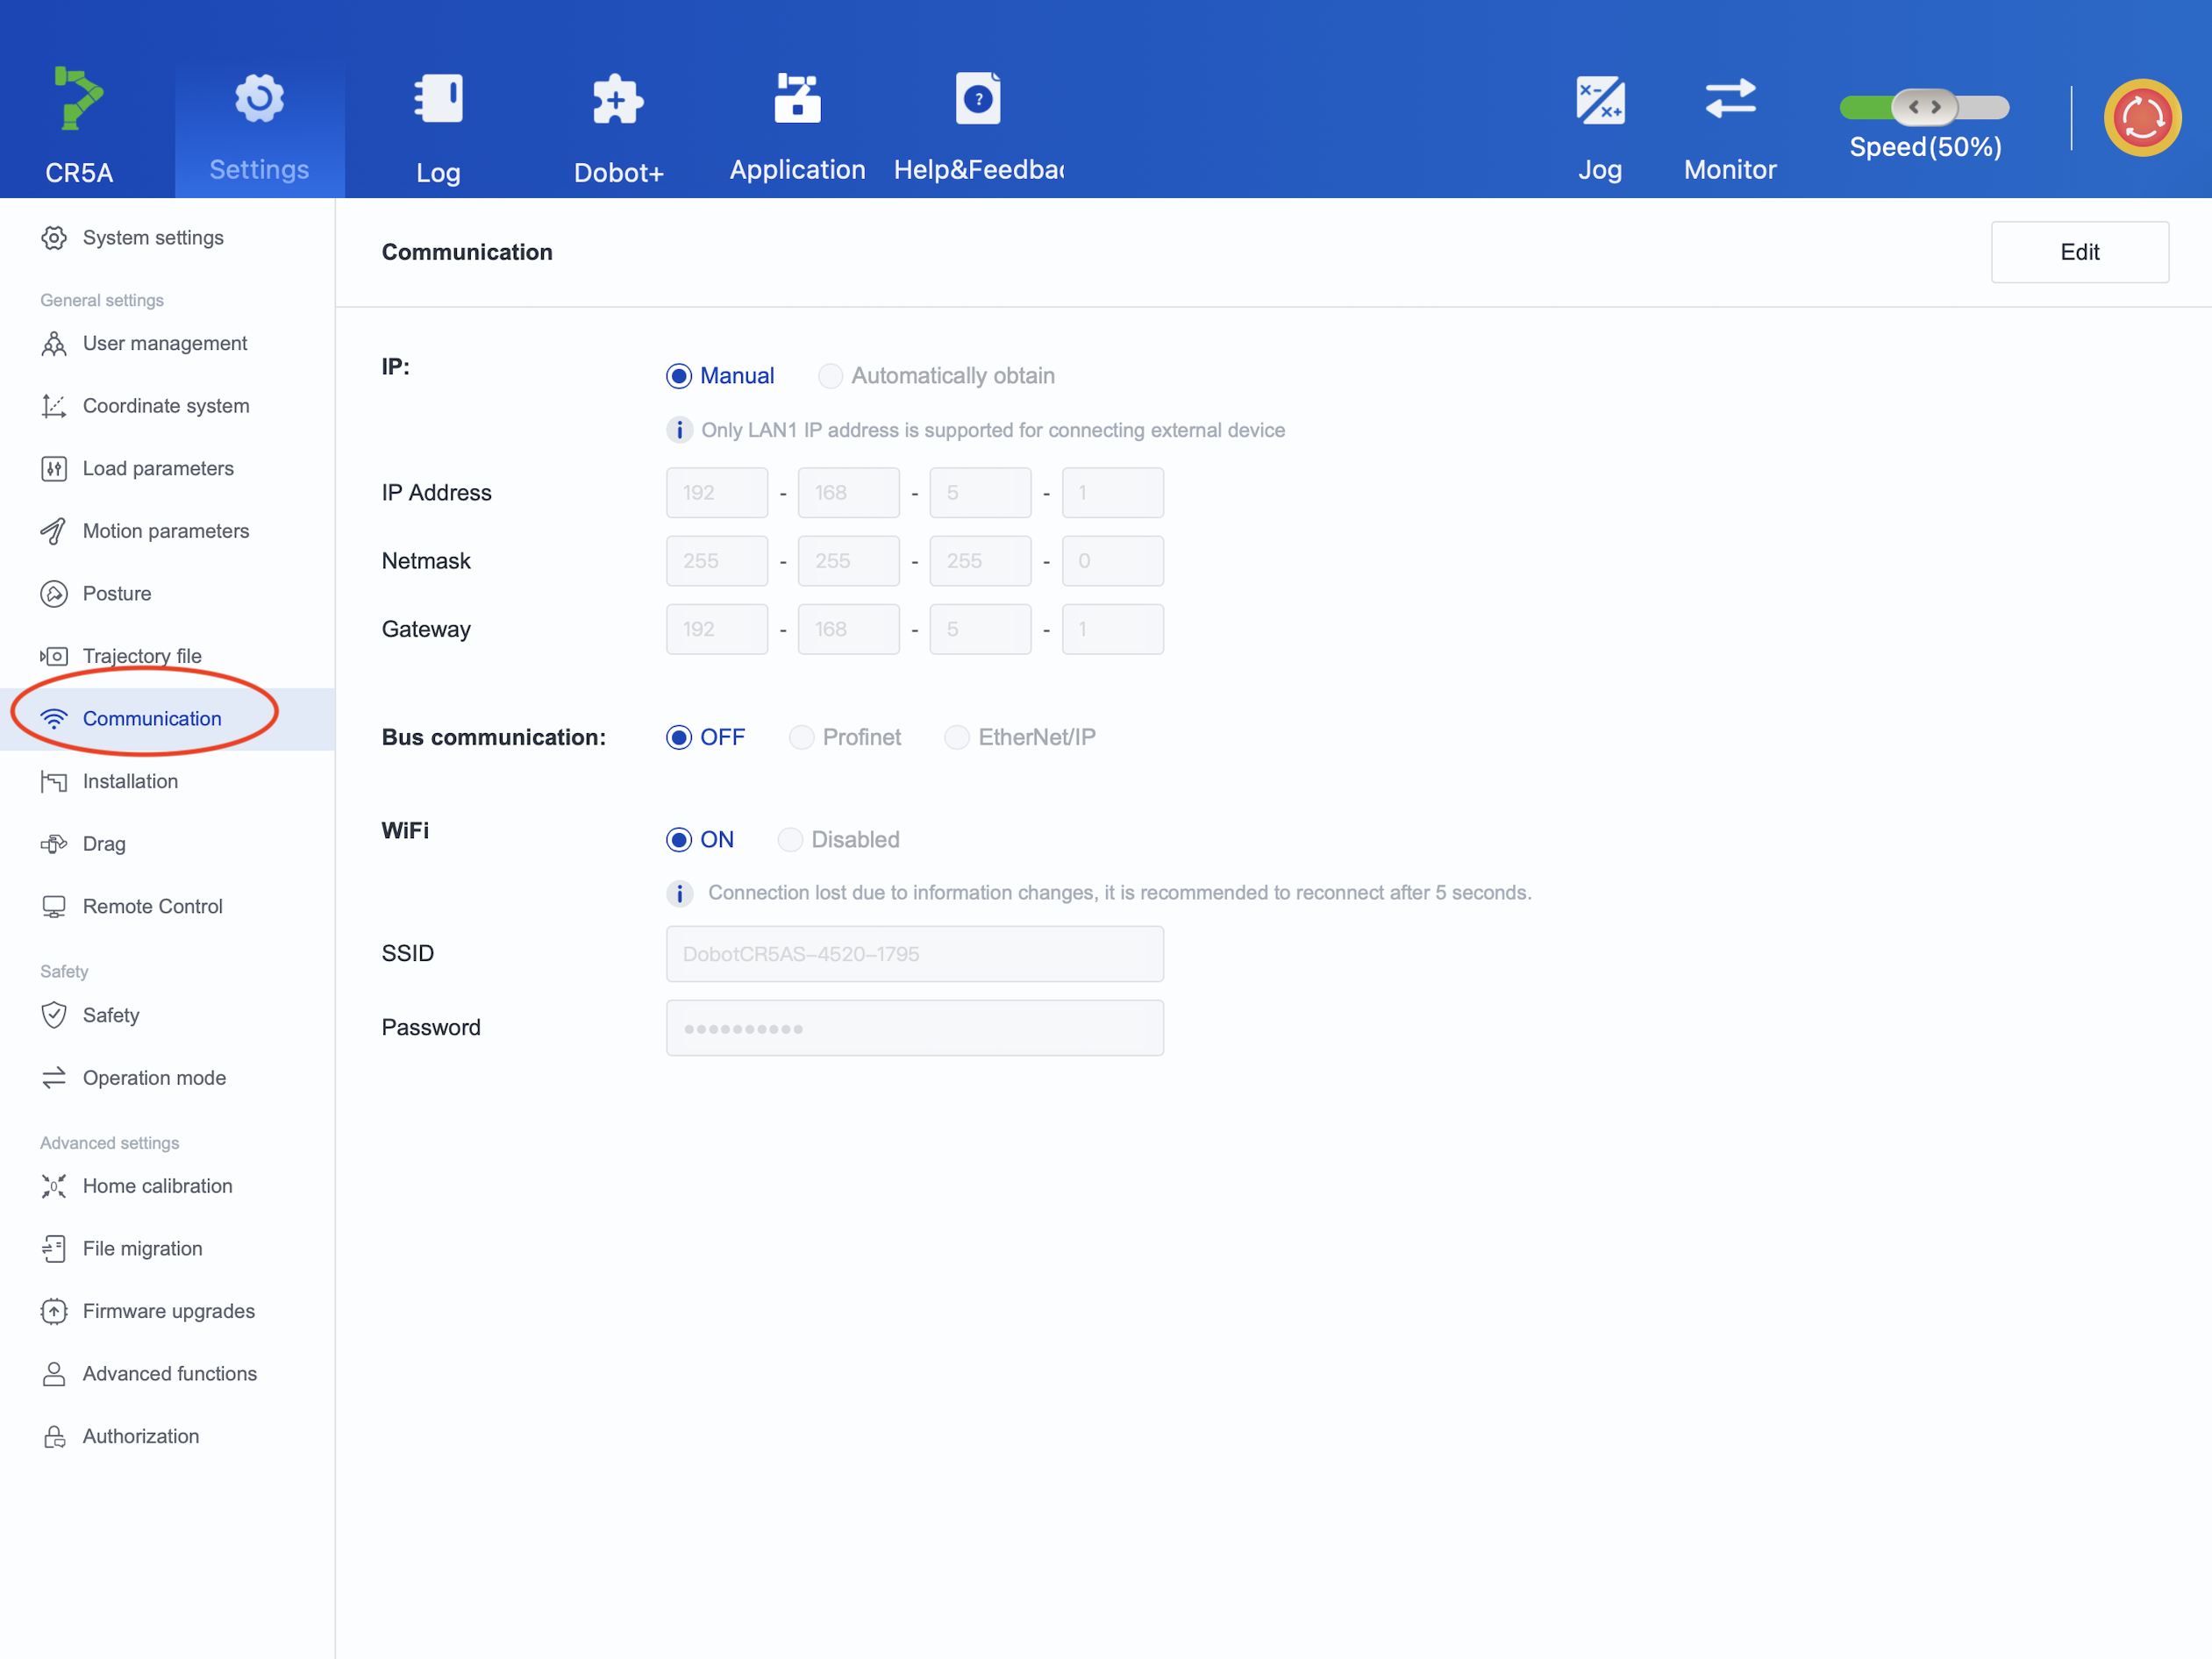
\includegraphics[width=0.9\textwidth]{10.png}
\end{figure}

\item By pressing ``Dobot+'' you'll be able to explore the extensions; some important ones are the Gripper and SafeSkin extensions.

\begin{figure}[H]
    \centering
    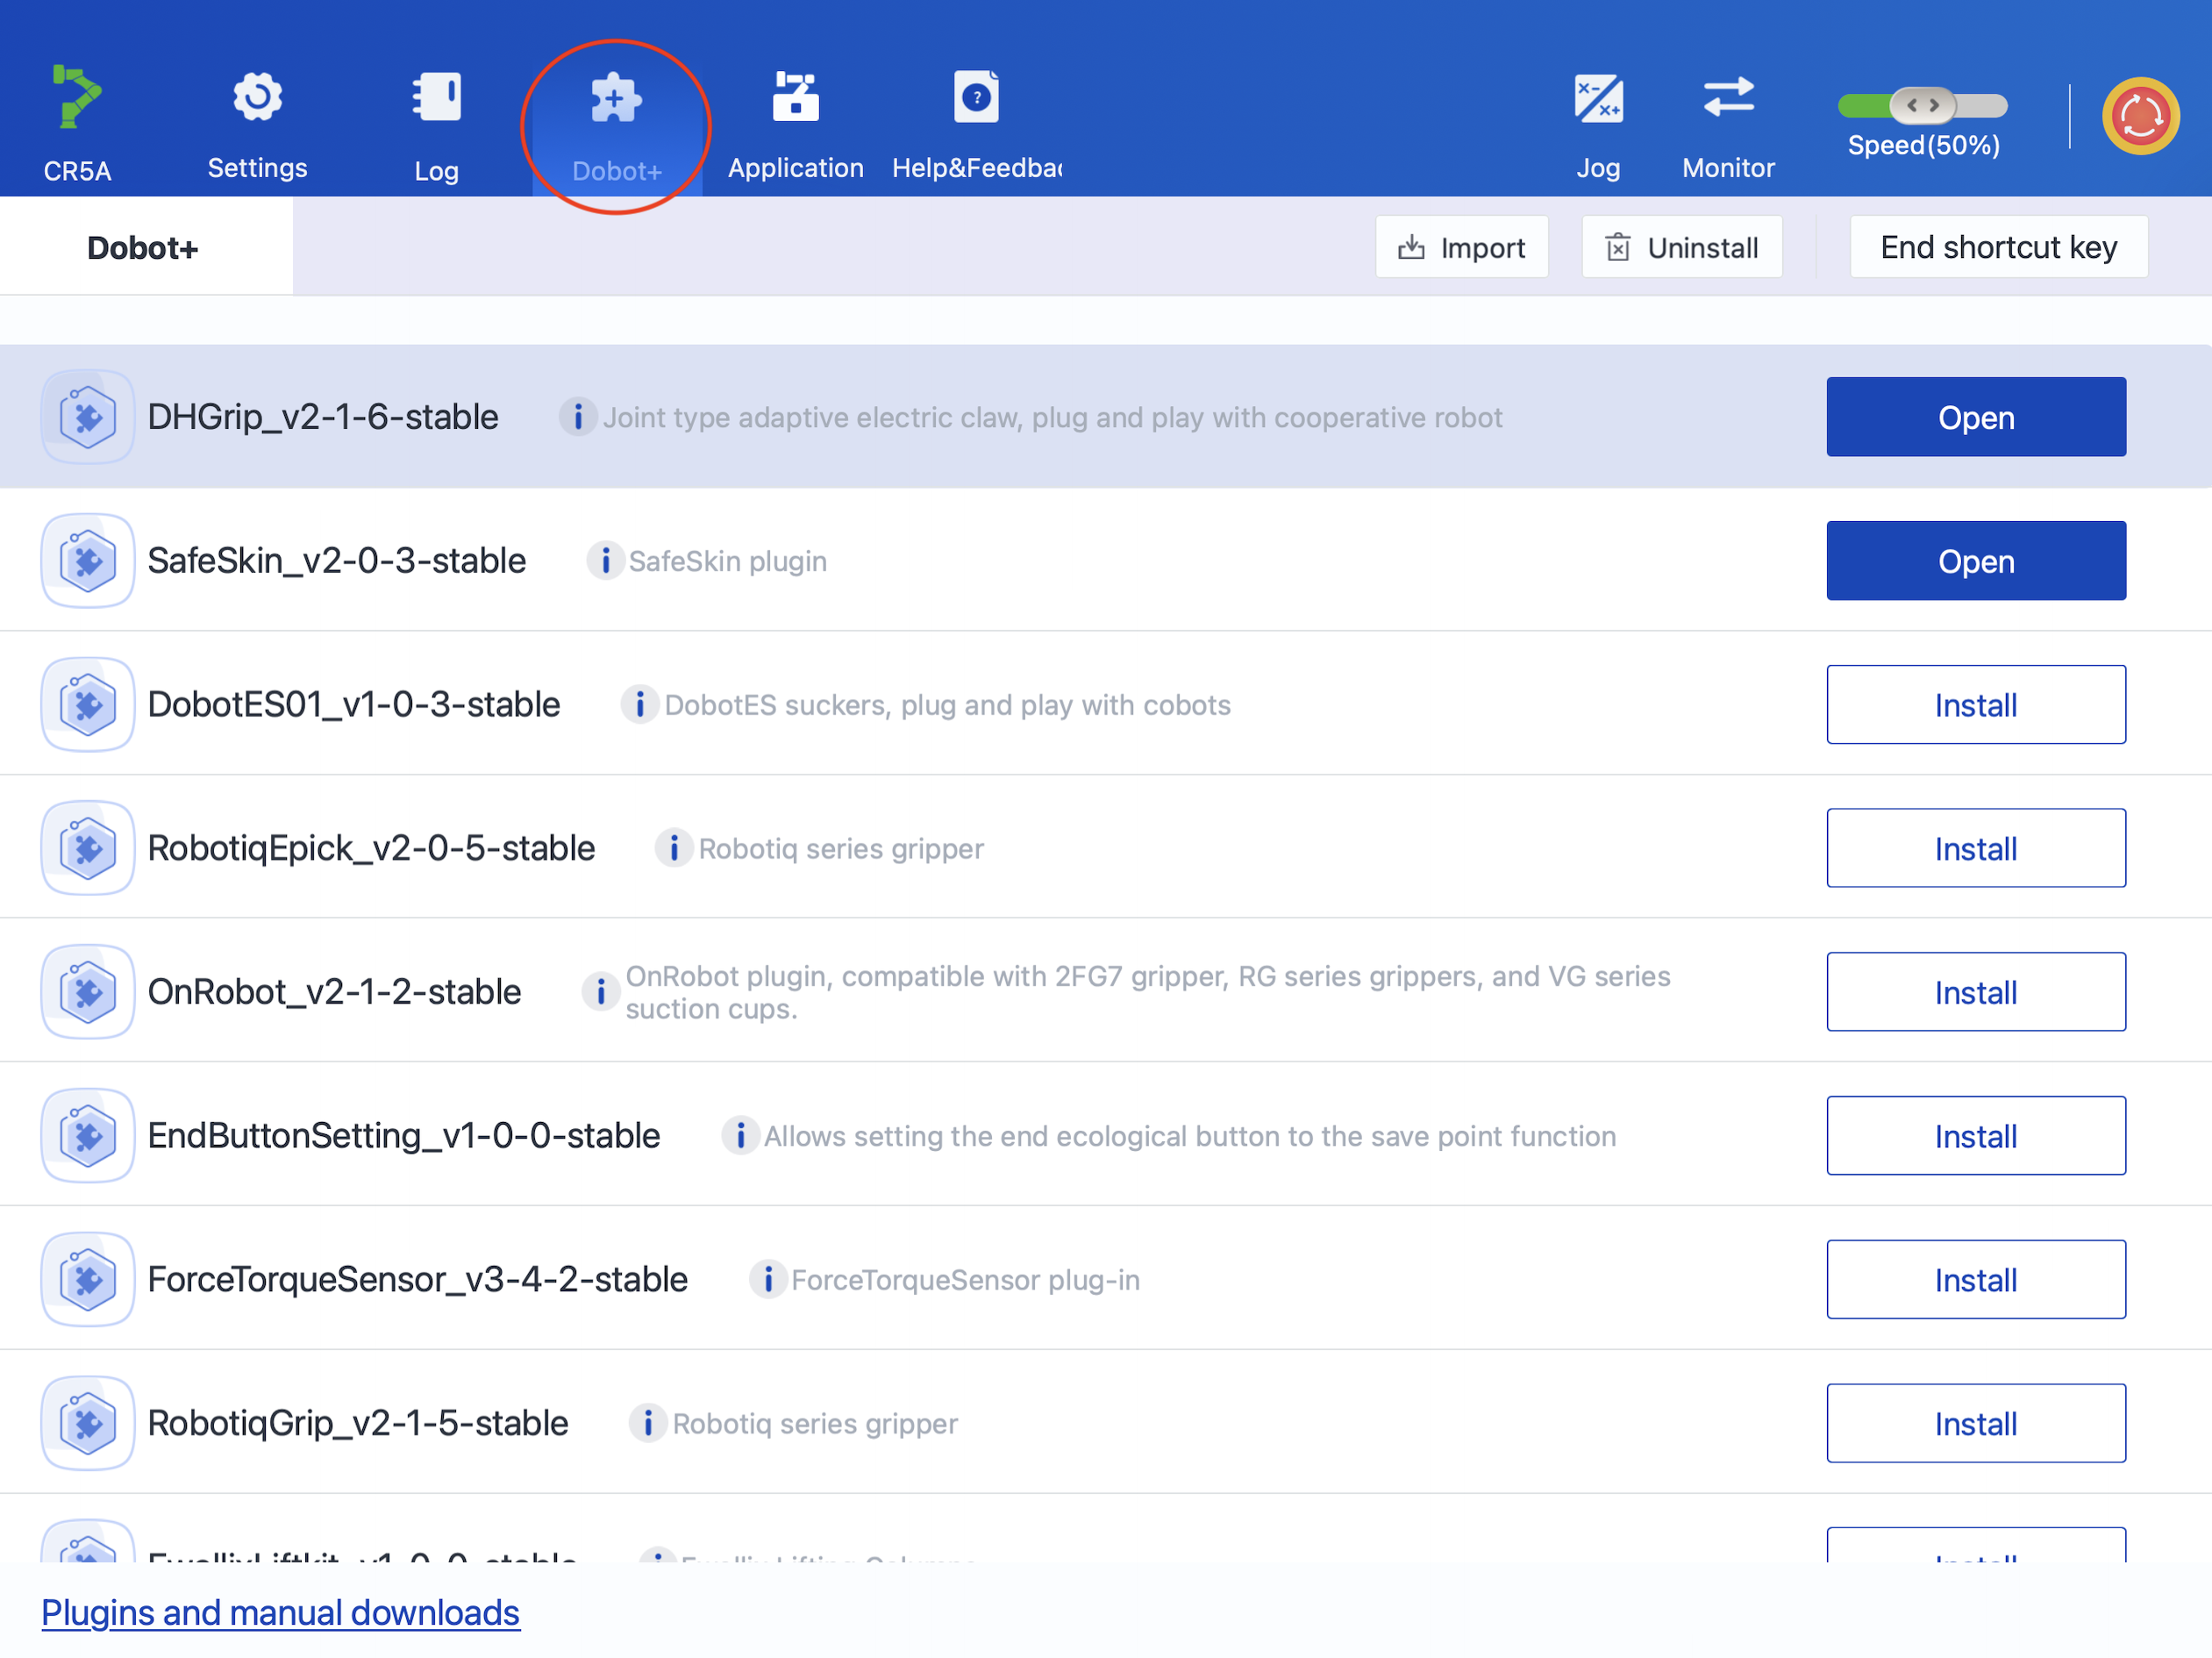
\includegraphics[width=0.9\textwidth]{11.png}
\end{figure}

\begin{figure}[H]
    \centering
    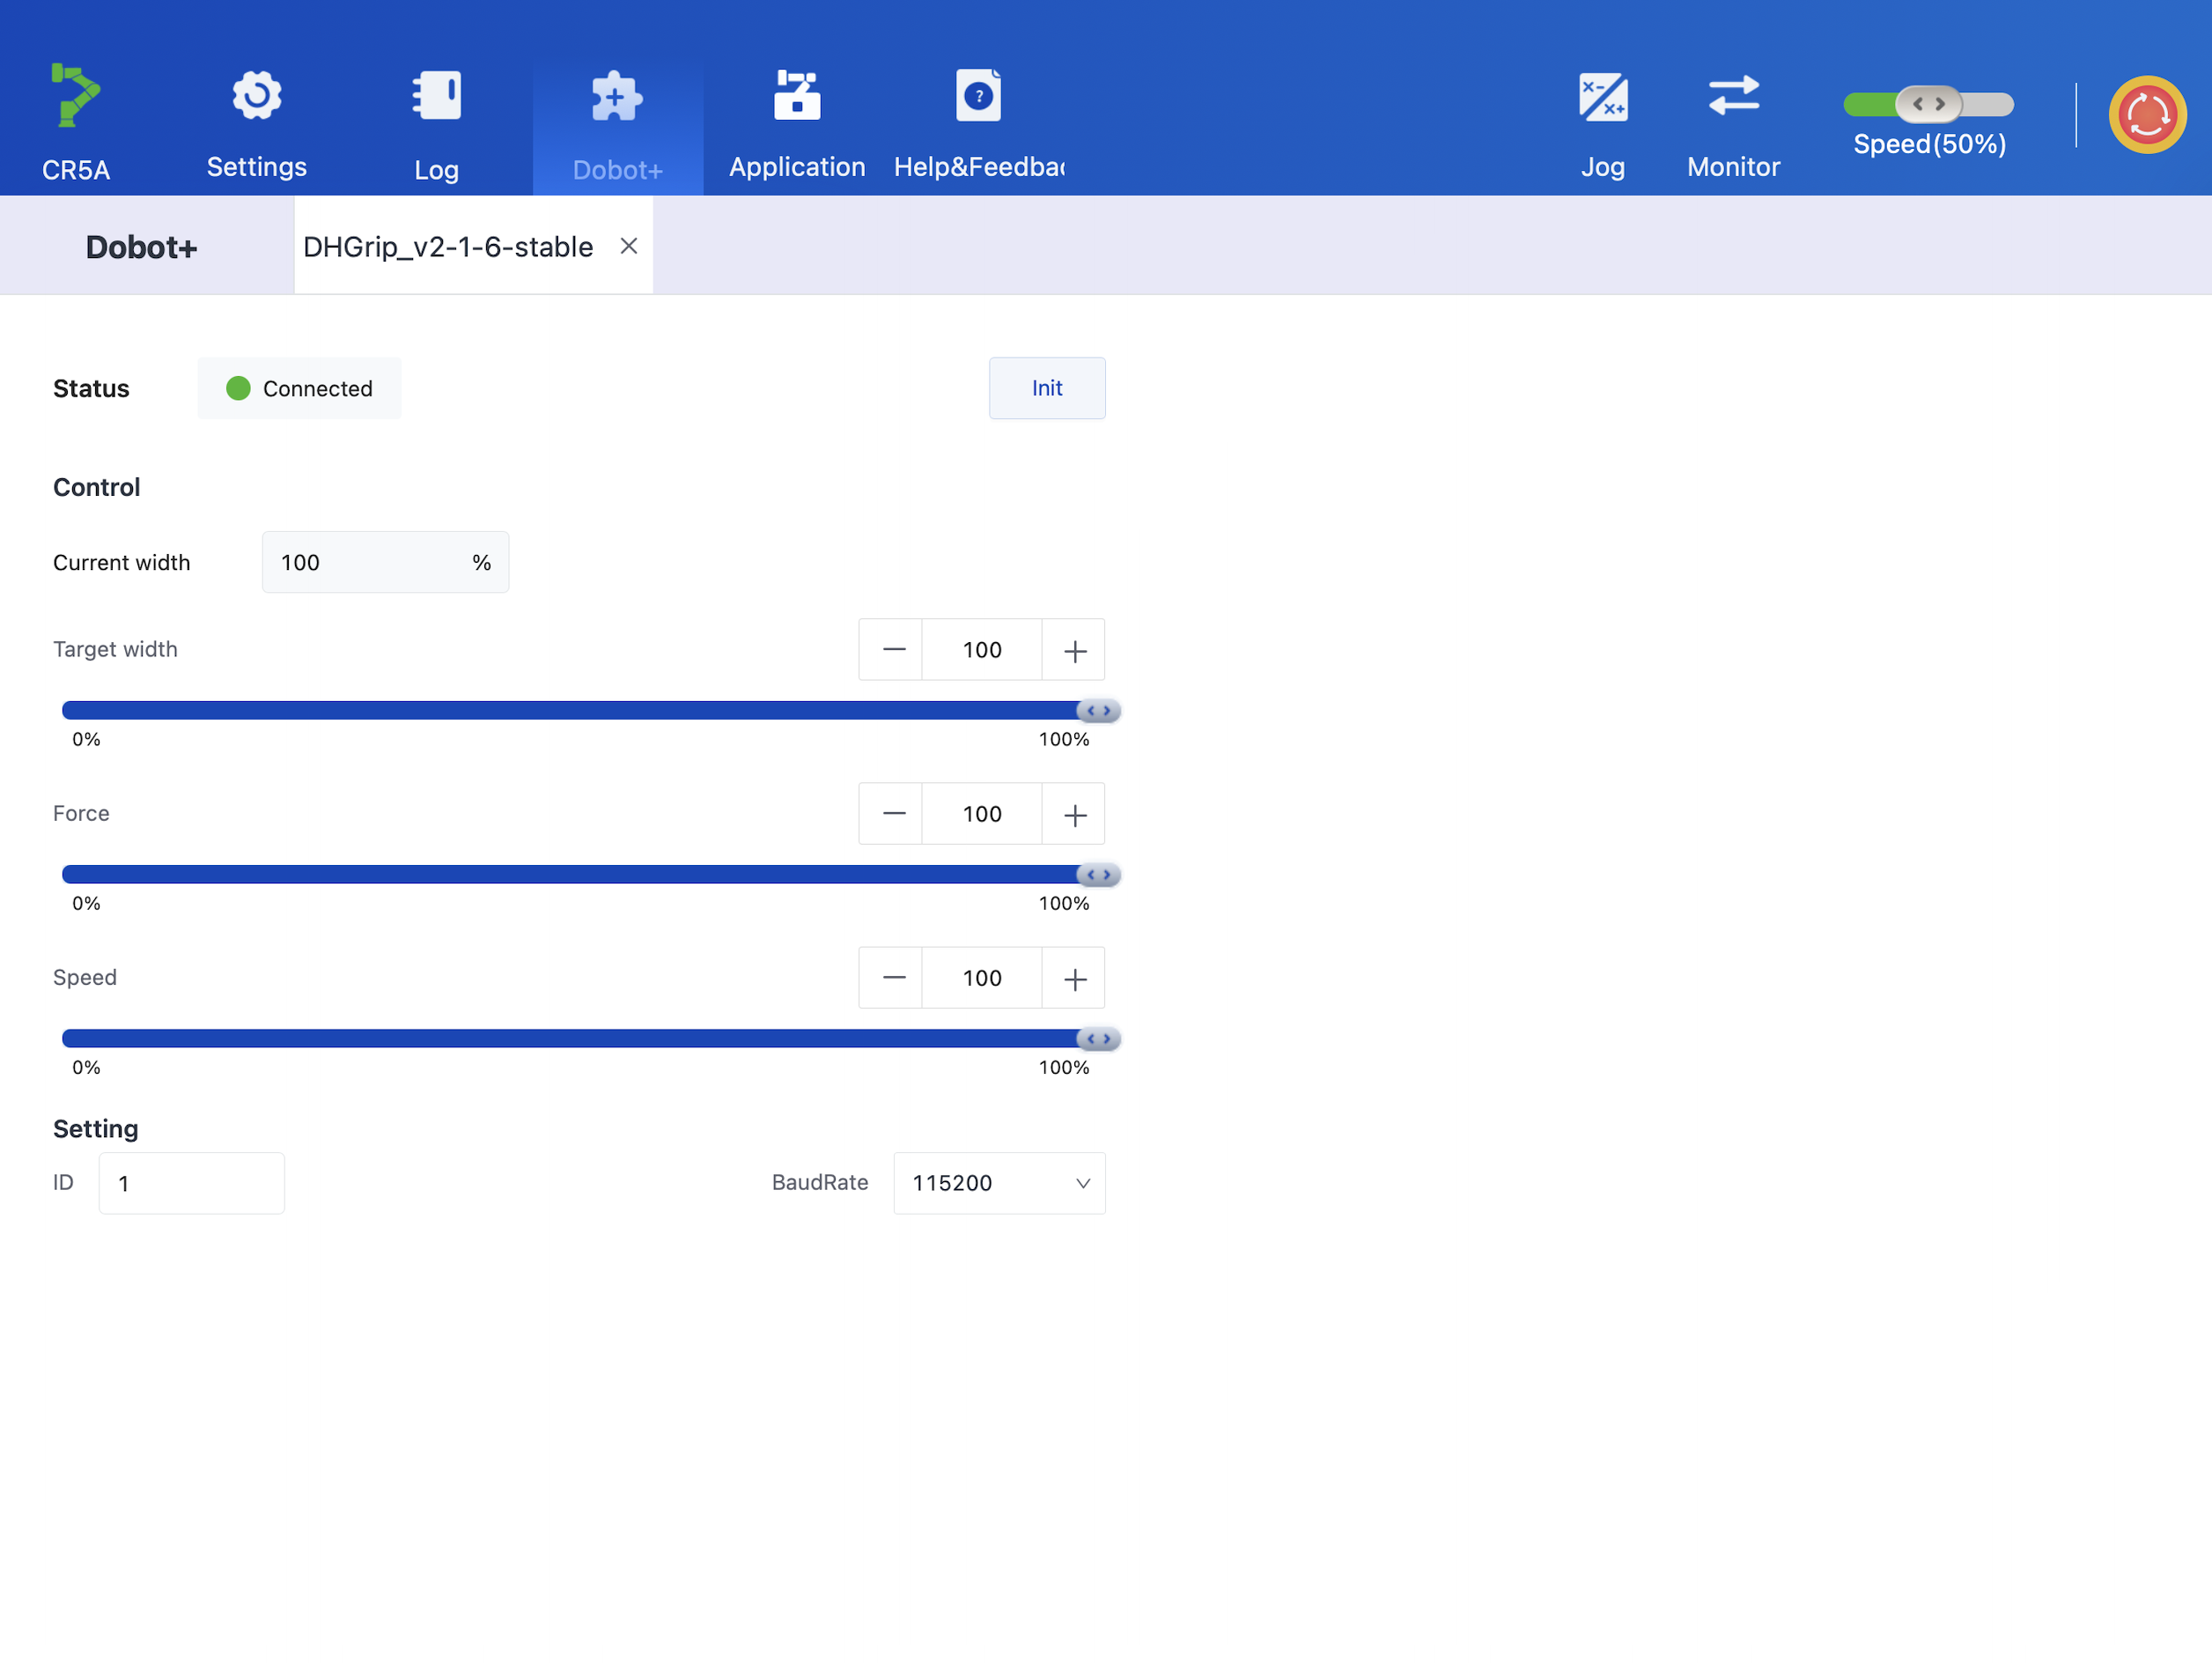
\includegraphics[width=0.9\textwidth]{12.png}
\end{figure}

\begin{figure}[H]
    \centering
    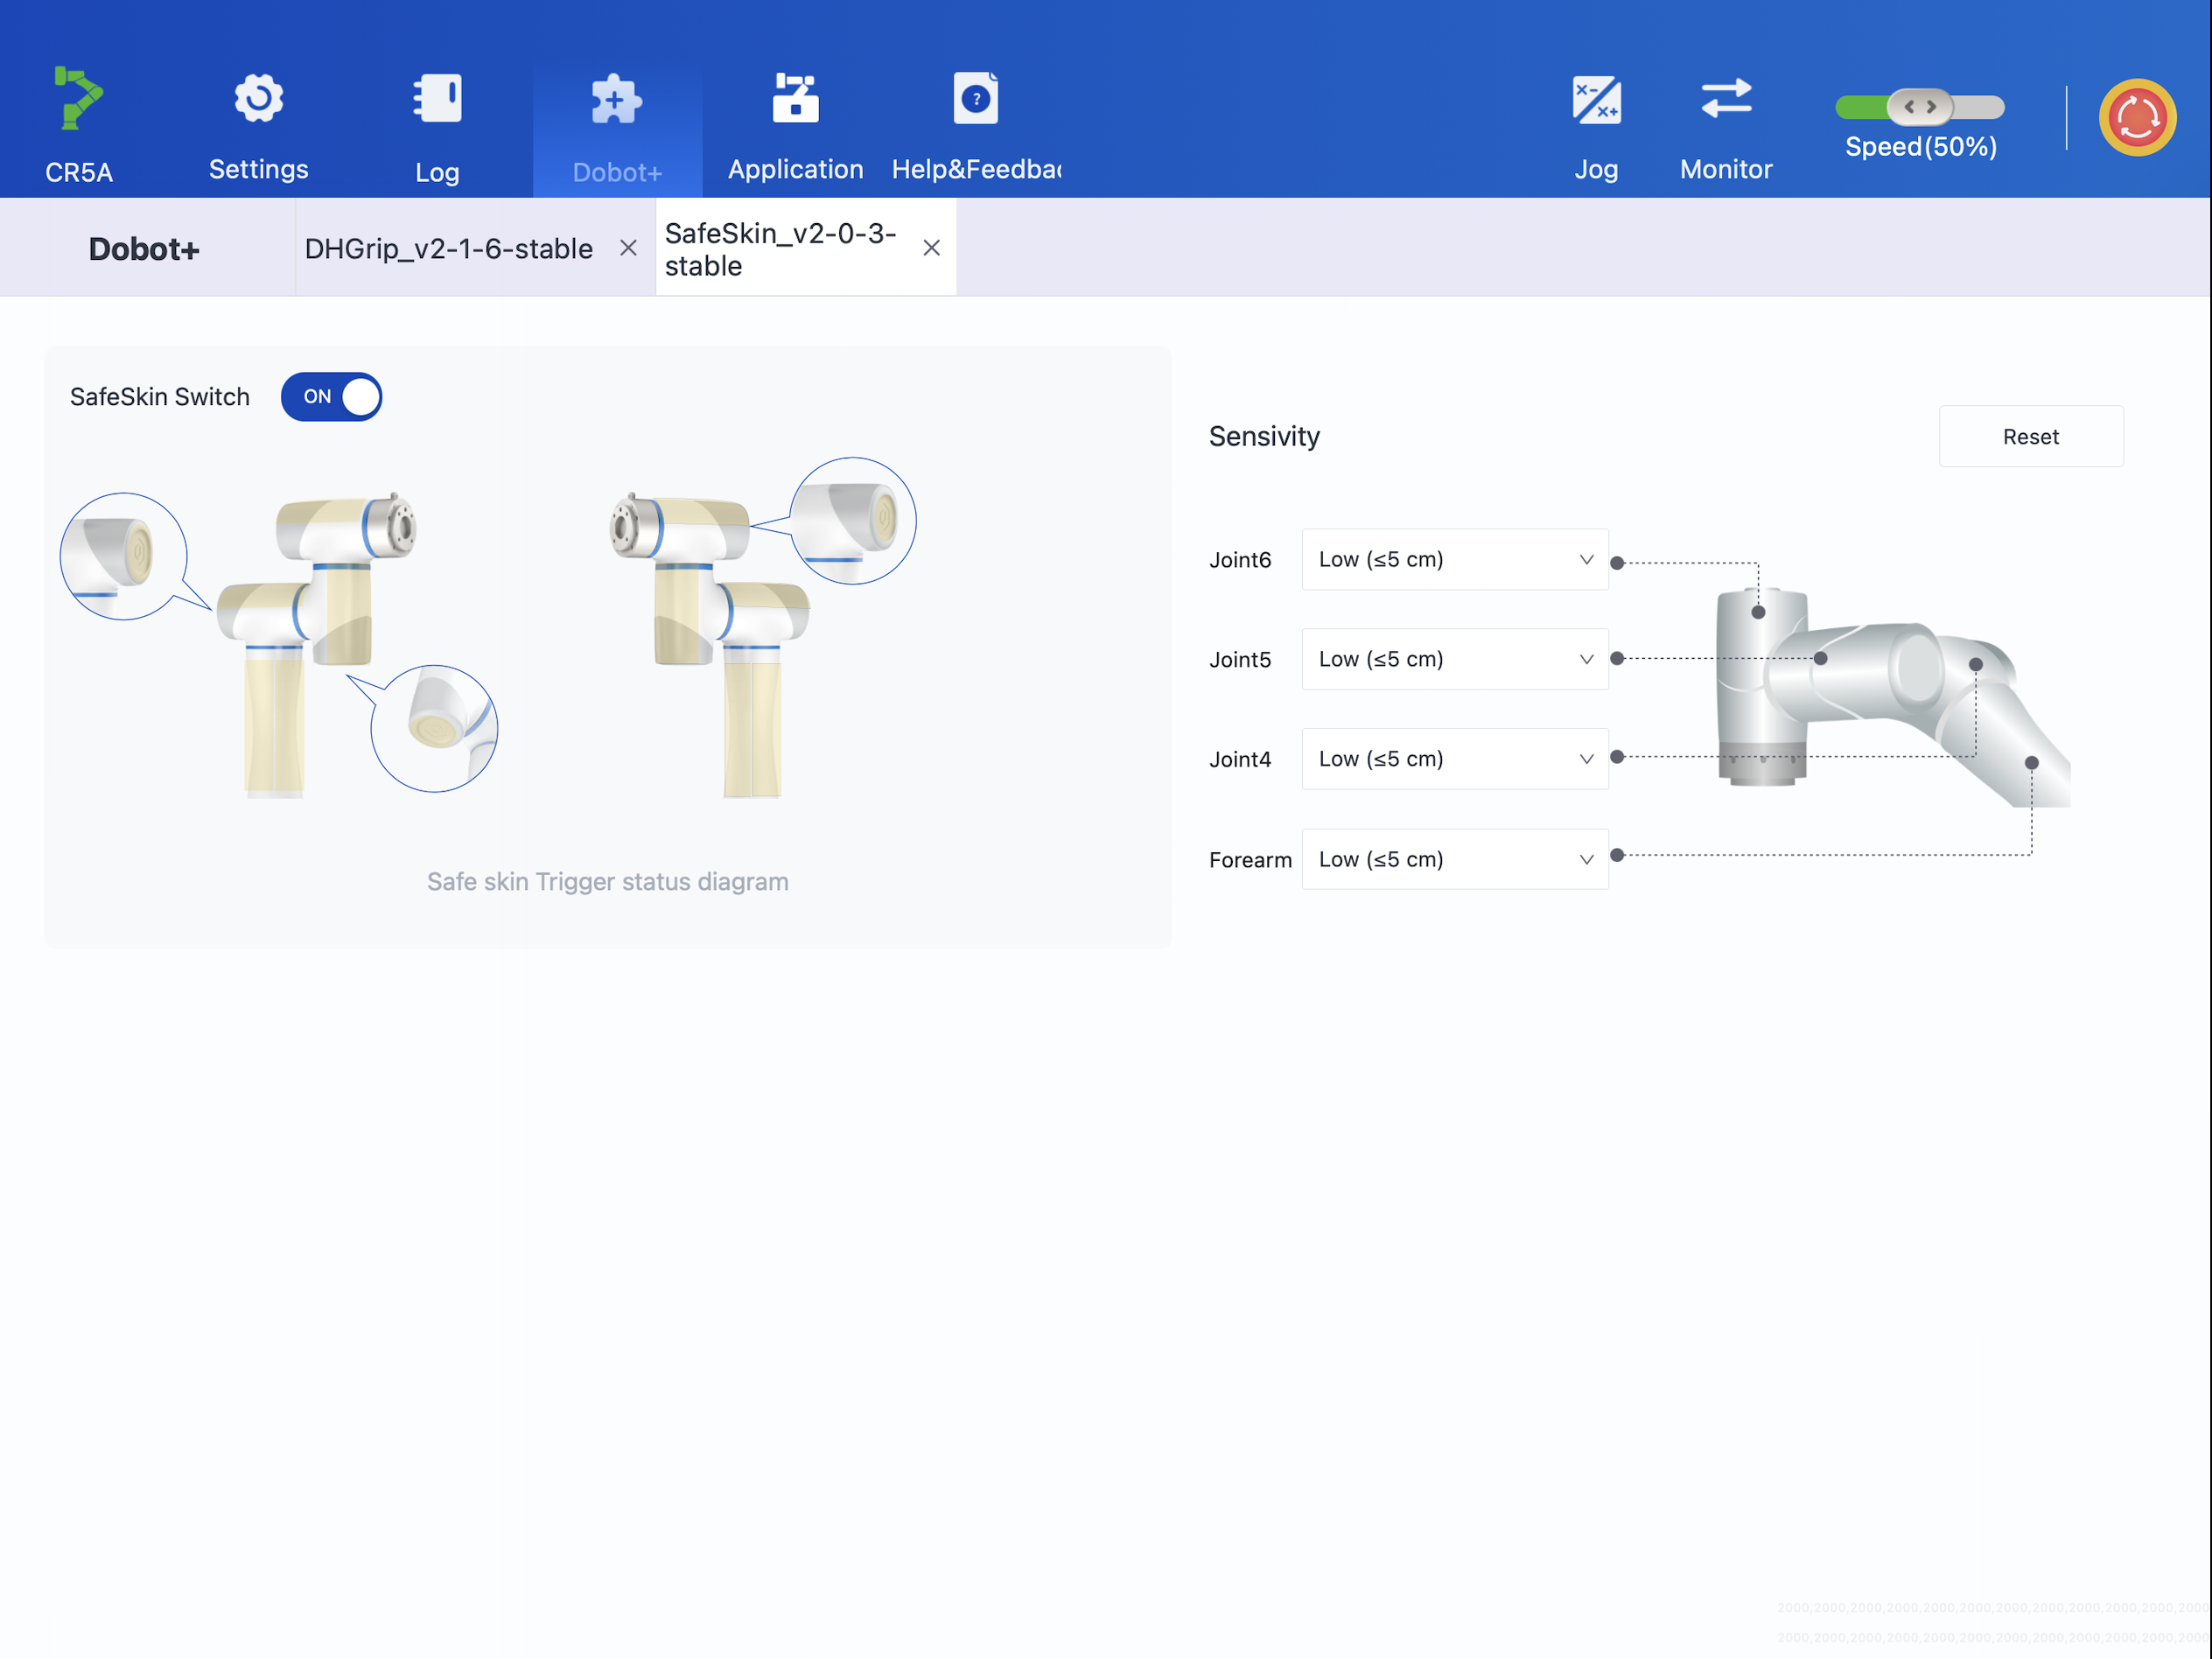
\includegraphics[width=0.9\textwidth]{13.png}
\end{figure}

\item By pressing ``Application'' you'll be able to program the Dobot using the software's functions. You have the option to do Blockly programming and Script programming. Both are valid and have the option ``Points'', which allows you to record points while in Drag Mode and use them in your script.

\begin{figure}[H]
    \centering
    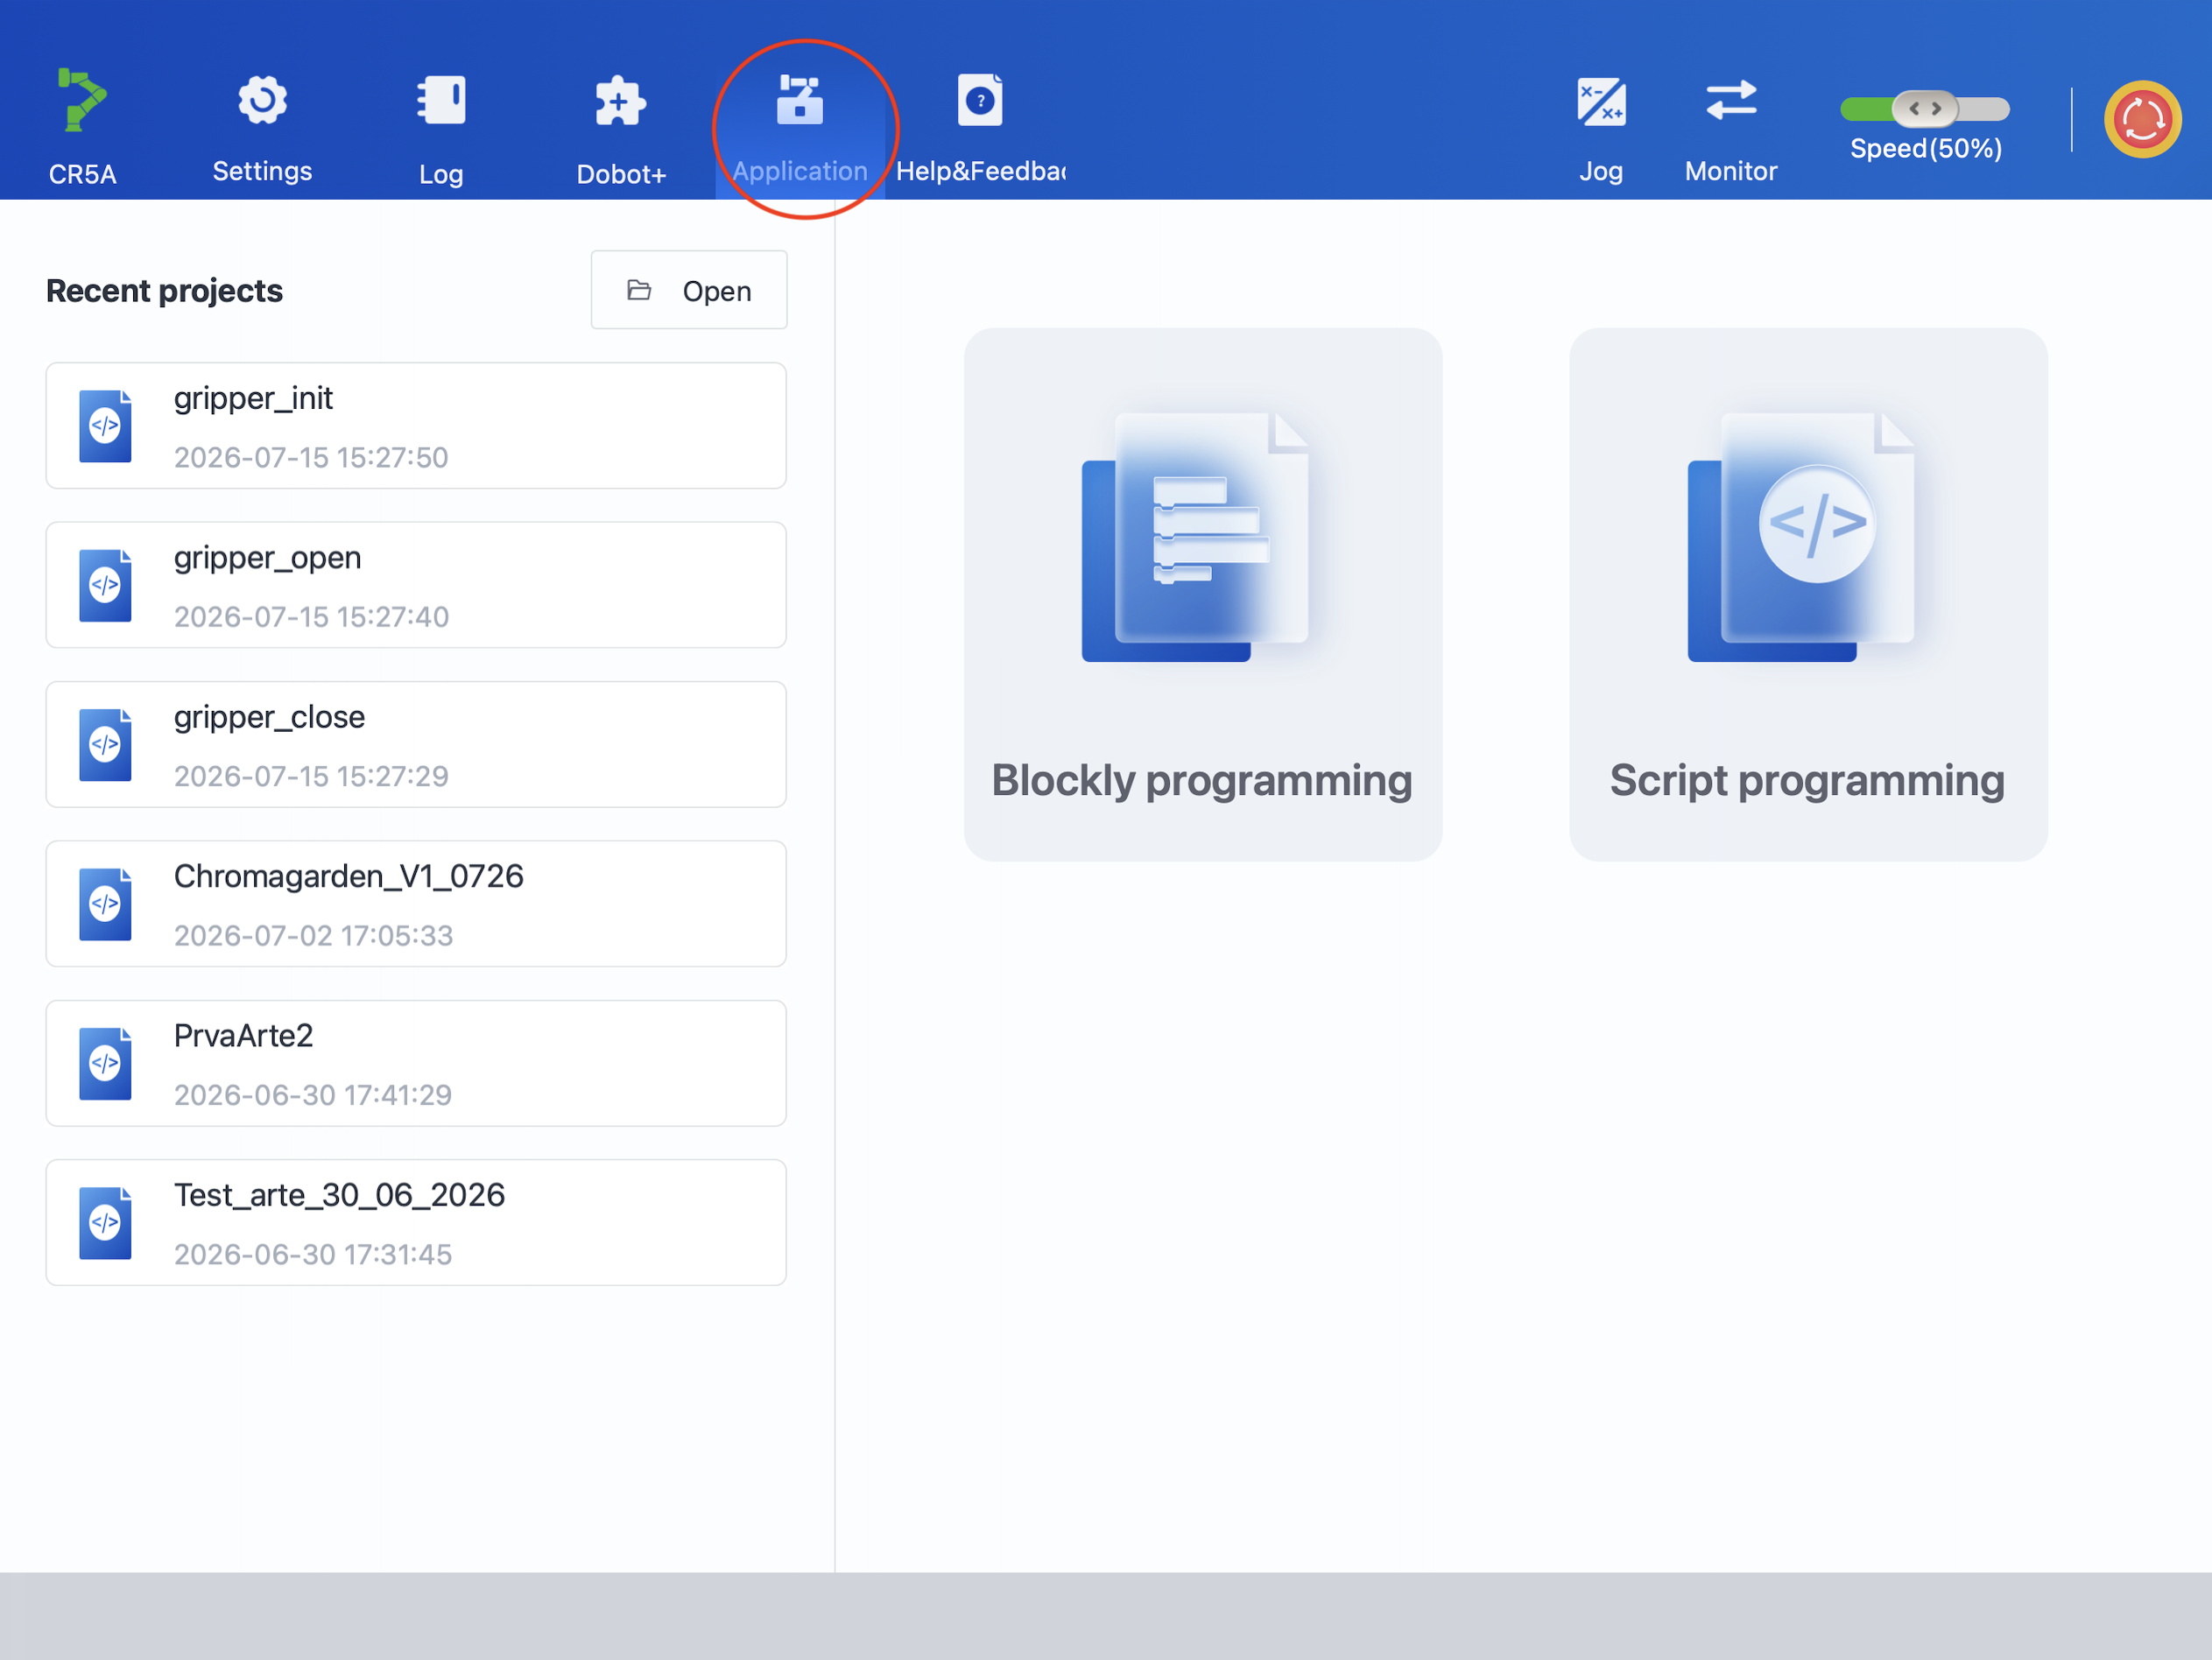
\includegraphics[width=0.9\textwidth]{14.png}
\end{figure}

\begin{figure}[H]
    \centering
    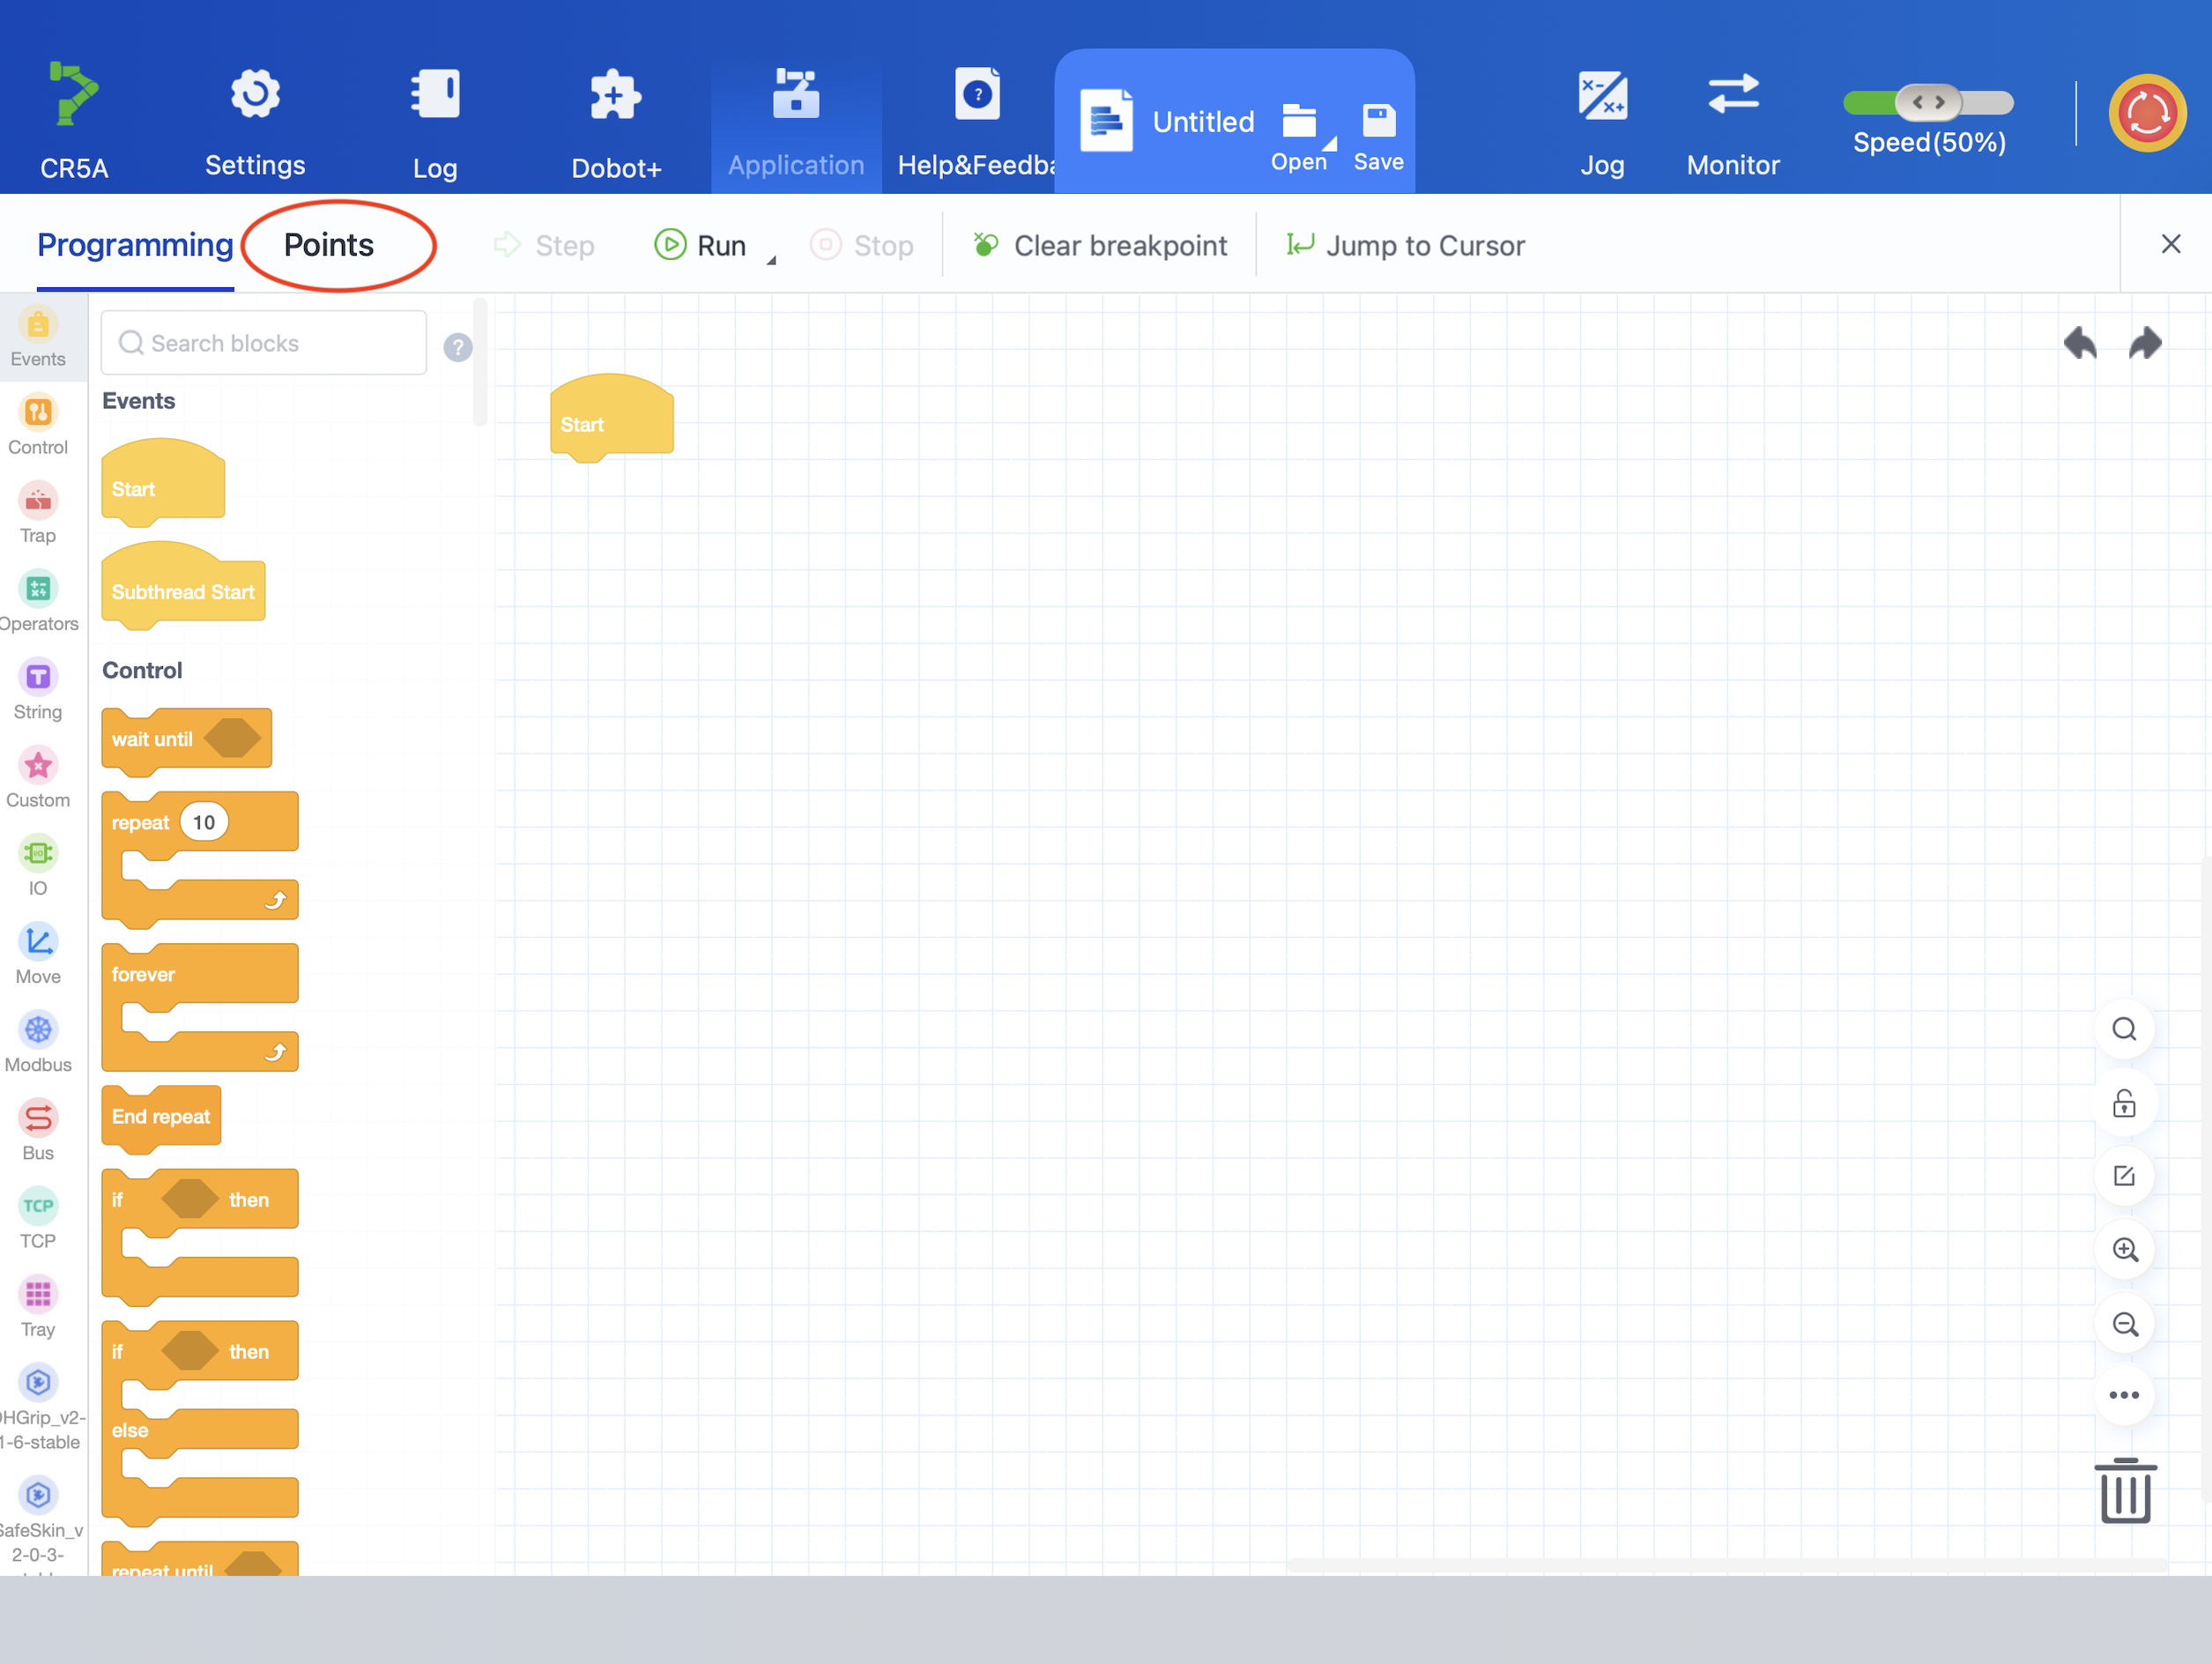
\includegraphics[width=0.9\textwidth]{15.png}
\end{figure}

\begin{figure}[H]
    \centering
    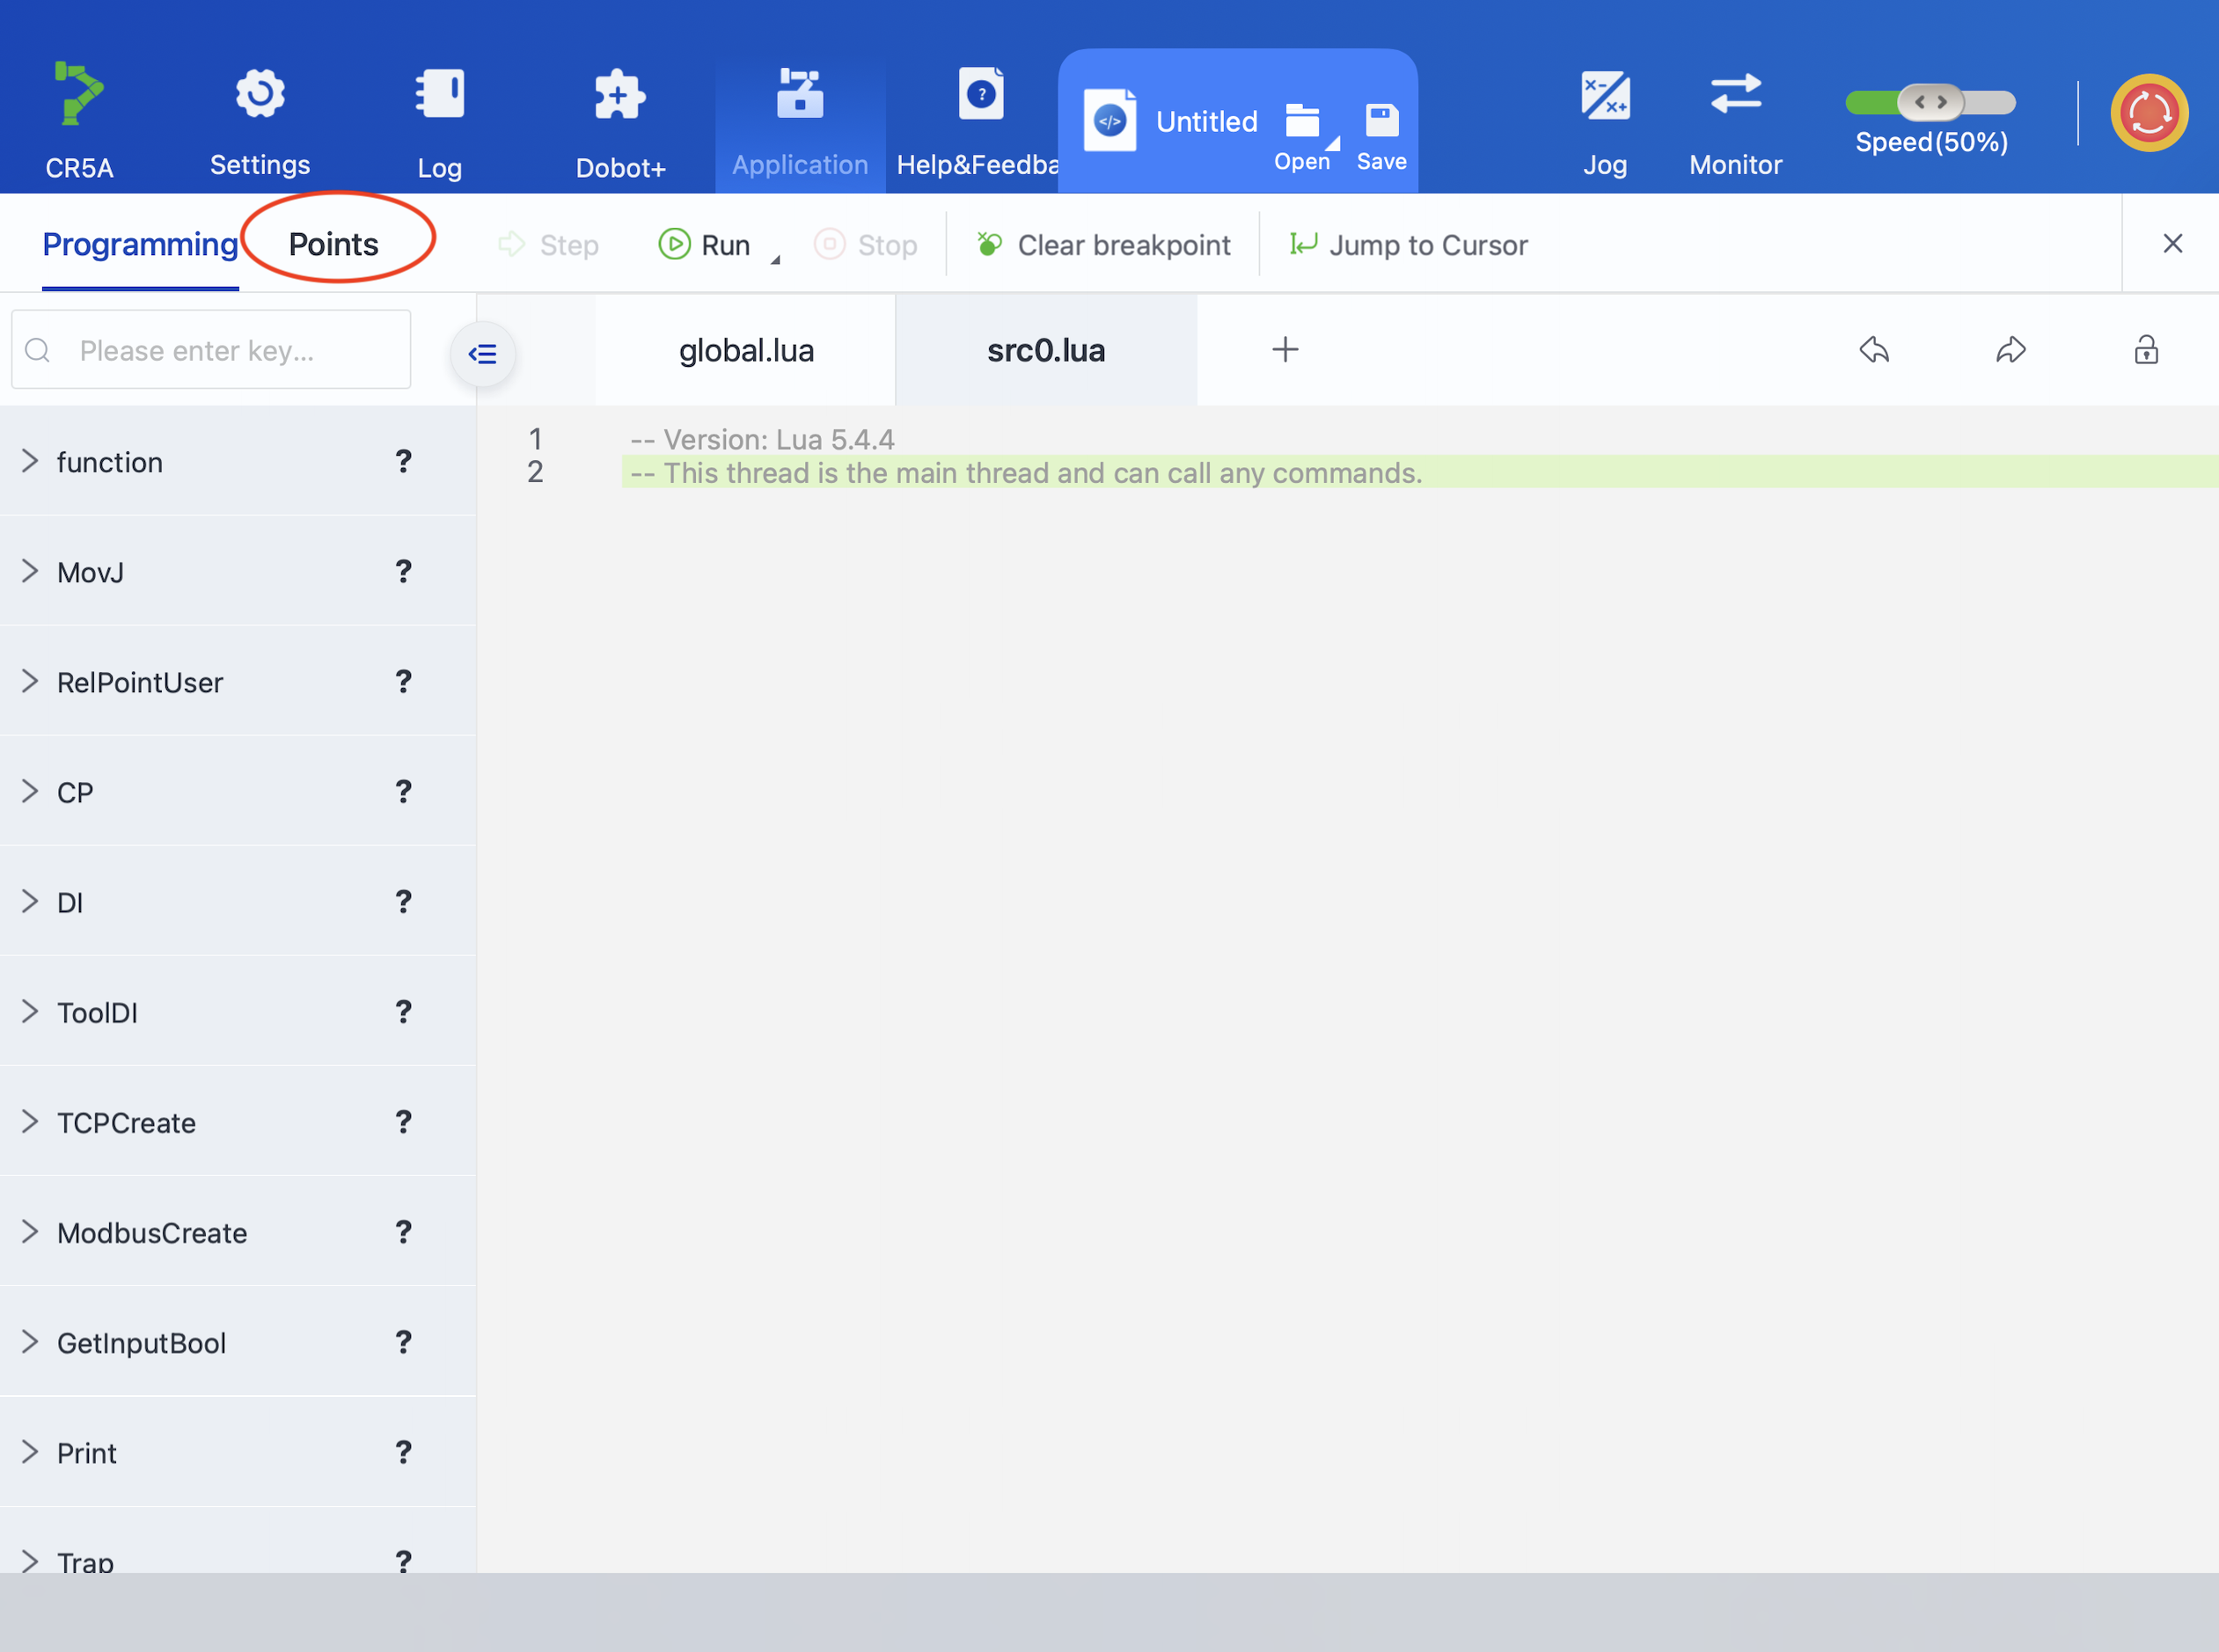
\includegraphics[width=0.9\textwidth]{16.png}
\end{figure}

\begin{figure}[H]
    \centering
    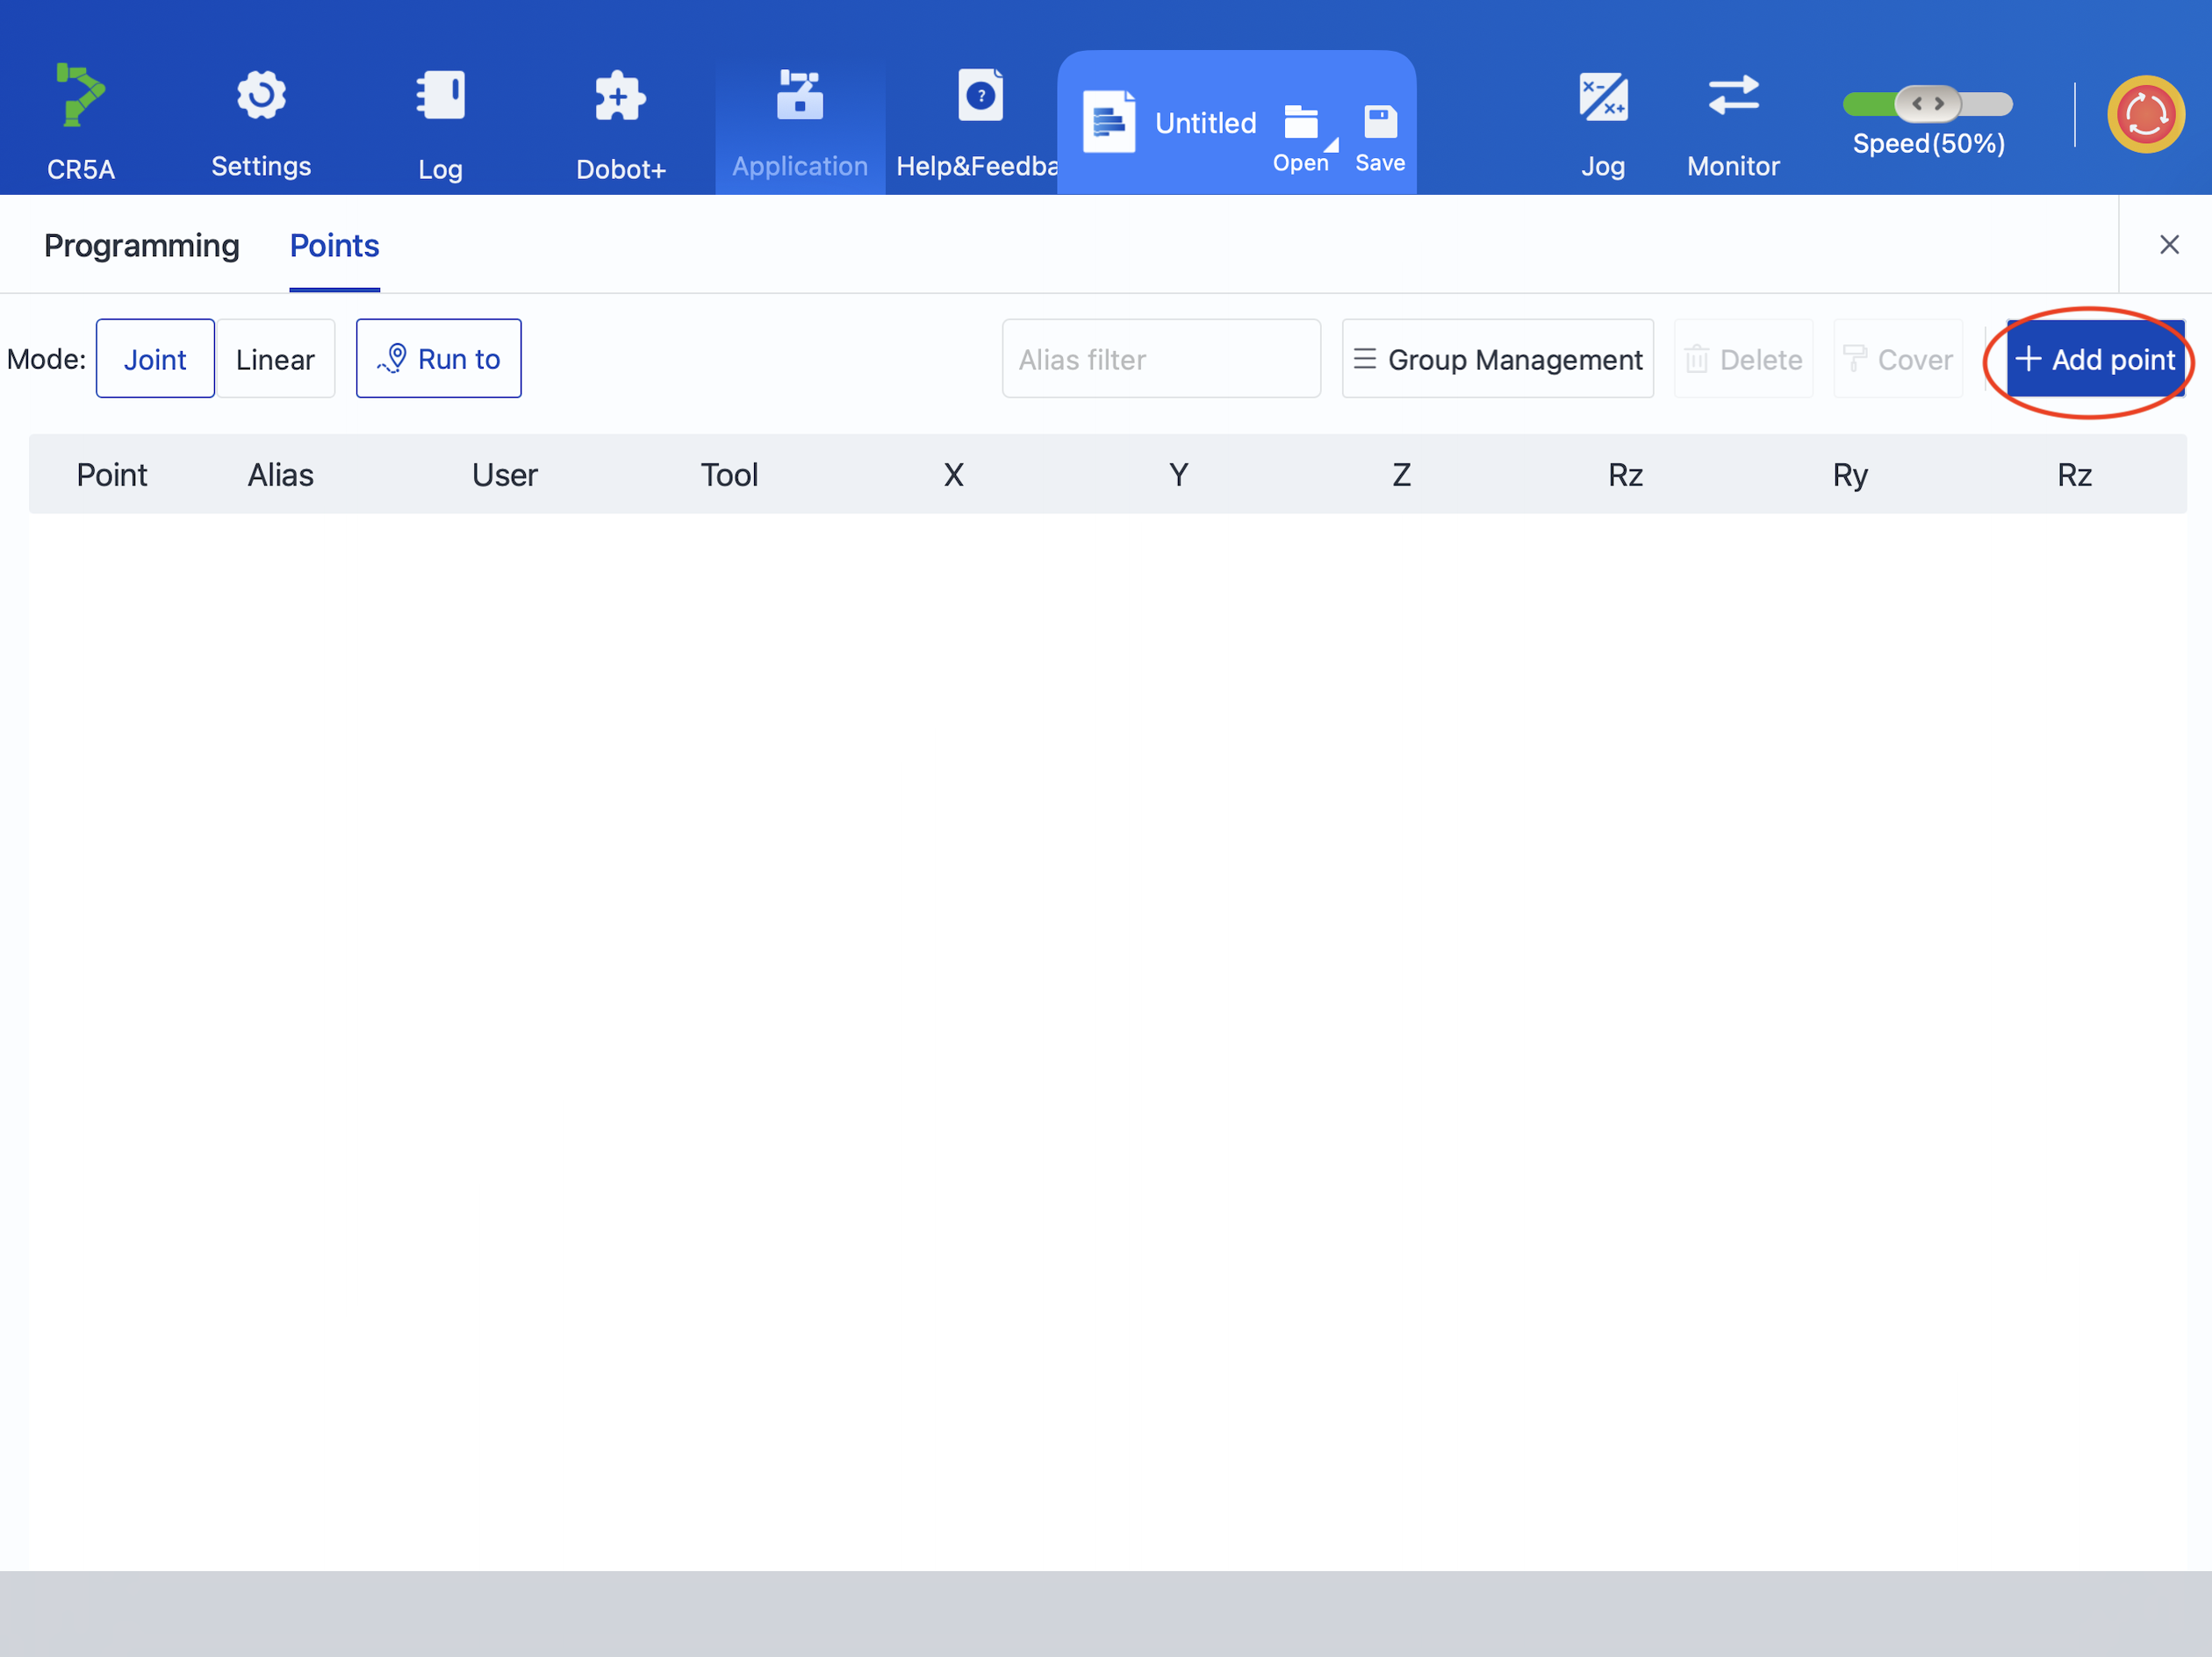
\includegraphics[width=0.9\textwidth]{17.png}
\end{figure}

\item Whenever the E-Stop button is pressed, or any other error occurs, you can view and clear these from the ``Log'' panel.

Please note that, whenever the E-Stop button is pressed, you'll have to disengage it, clear the alarm, and then go back to the ``CR5A'' panel to Enable the Dobot again.

\begin{figure}[H]
    \centering
    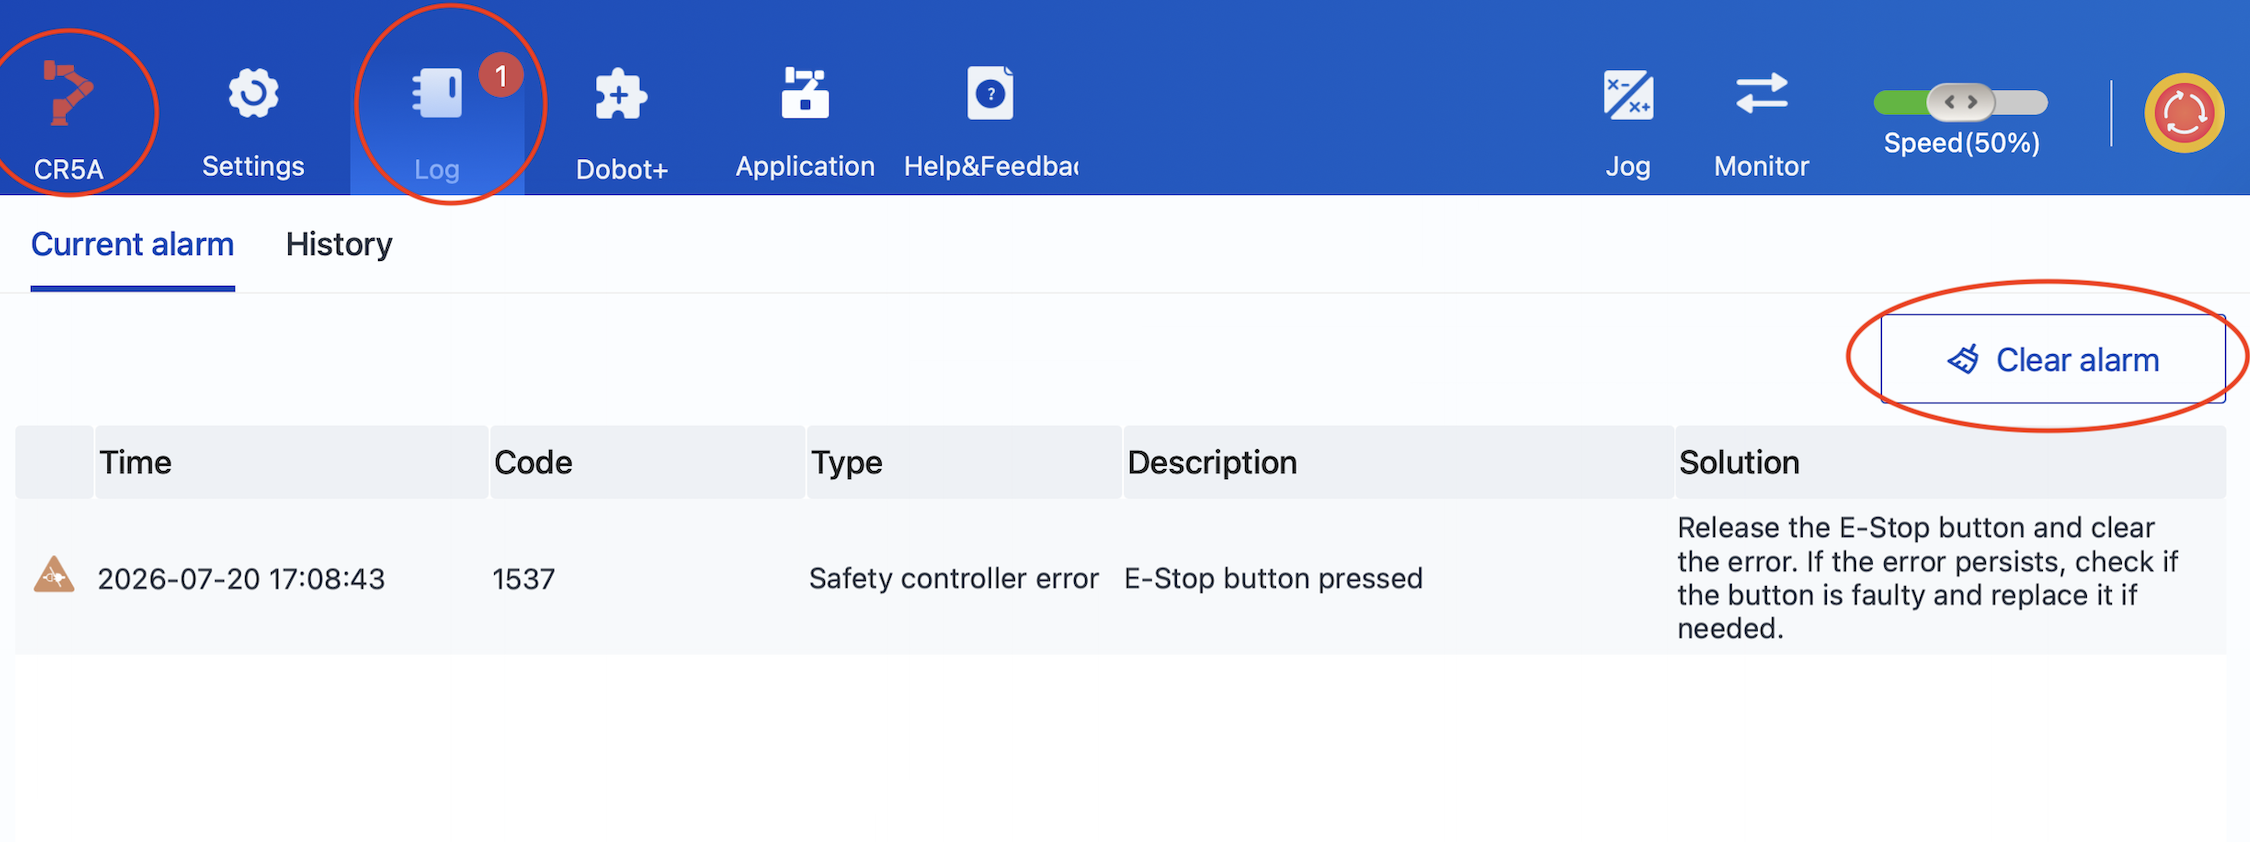
\includegraphics[width=0.9\textwidth]{18.png}
\end{figure}

\end{itemize}

% ============================================================
\section{How to program with Python scripts}
\label{sec:python-programming}
% ============================================================

Following is a brief explanation of the main features and commands that allow you to control the Dobot via scripts in TCP mode.

The library I decided to use is the official one; it's available on GitHub at \url{https://github.com/Dobot-Arm/TCP-IP-Python-V4}, but I have also put it into the repository this manual is attached to.

Here is a list of all the commands that could be helpful:

\subsubsection*{Connection / power state}
\begin{itemize}[leftmargin=1.2cm]
    \item \code{EnableRobot()} --- powers up the arm
    \item \code{DisableRobot()} --- powers it down
    \item \code{ClearError()} --- resets alarm state
\end{itemize}

\subsubsection*{Motion}
\begin{itemize}[leftmargin=1.2cm]
    \item \code{MovJ()} --- joint-space point-to-point move
    \item \code{MovL()} --- linear (Cartesian) move
    \item \code{StartDrag()} --- enters drag/teach mode (manual hand-guiding)
    \item \code{StopDrag()} --- exits drag mode
    \item \code{SpeedFactor()} --- sets global speed ratio
\end{itemize}

\subsubsection*{Status / feedback}
\begin{itemize}[leftmargin=1.2cm]
    \item \code{RobotMode()} --- returns current robot state (enabled, running, error, etc.)
    \item \code{GetAngle()} --- reads current joint angles
    \item \code{GetPose()} --- reads current Cartesian position
\end{itemize}

\subsubsection*{Kinematics}
\begin{itemize}[leftmargin=1.2cm]
    \item \code{InverseKin()} --- converts a Cartesian target into joint angles
\end{itemize}

\subsubsection*{Gripper / tool I/O}
\begin{itemize}[leftmargin=1.2cm]
    \item \code{SetToolPower()} --- turns tool-side power on/off (used before gripper control)
    \item \code{ToolDOInstant()} --- toggles a tool digital output instantly, used to open/close the gripper
    \item \code{GetToolDO()} --- reads current tool digital output state
\end{itemize}

\subsubsection*{Modbus (for grippers that use it, like DH Robotics PGC-140-50)}
\begin{itemize}[leftmargin=1.2cm]
    \item \code{ModbusRTUCreate()} --- opens a Modbus RTU connection to the gripper (slave ID, baud rate, parity, data bits, stop bits)
    \item \code{ModbusClose()} --- closes that Modbus connection
\end{itemize}

To control a DH gripper you can either use the Modbus protocol (it's not advised, since you'd have to have the gripper connected to the Dobot's main computer with a cable that is not always included) or use the Remote Control protocol, which has the Python code run prewritten scripts in DobotStudio Pro. The latter is the best option and only requires an initial setup that can be cumbersome, but is much easier to use afterward.

\subsection*{Remote control for the DH Gripper}

\textbf{Setup:}

\begin{enumerate}[leftmargin=1.2cm]
    \item Disable TCP mode.
    \item Connect the Dobot to DobotStudio Pro.
    \item Download the DH gripper plug-in from the list provided in the software.
    \item In the programming section of the software, add the 3 main scripts (they are included in the ``Examples'' folder, in a folder that specifies those are the Lua scripts connected to Example 11, which moves the gripper).
    \item Enable TCP mode. You will now be able to activate these 3 scripts as needed (see the ``Examples'' folder for the code structure). The only caveat is that you need to have the DobotStudio Pro software always open in the background, otherwise it will not work properly.
\end{enumerate}

I have added an example file in the GitHub repository for each of these, in the folder ``Examples''. To run these correctly, download the ``Examples'' folder, unzip it, and run the file you're interested in. The Dobot library was already included in this folder for easy use. With other libraries, you can just download them onto your PC and don't have to reference them every time, but this library doesn't have a \code{setup.py} file, so that can't be done here.

\begin{longtable}{@{}p{5cm}p{9.5cm}@{}}
\toprule
\textbf{Example file} & \textbf{What it does} \\
\midrule
\endhead
\code{00_hello_world.py} & Connects, enables the robot, and moves J1 back and forth from 0\textdegree{} to +/- 30\textdegree{} in order to show the basic connect $\rightarrow$ enable $\rightarrow$ move $\rightarrow$ disable pattern. \\ \midrule
\code{01_connect_and_status.py} & Connects, clears errors, enables the robot, and reads its current status via \code{RobotMode()}. \\ \midrule
\code{02_joint_motion.py} & Demonstrates \code{MovJ()} joint-space motion, moving J1 to 30\textdegree{} and reading joint angles before/after with \code{GetAngle()}. \\ \midrule
\code{03_linear_motion_and_pose.py} & Demonstrates \code{MovL()} straight-line motion, lifting the tool 50mm in Z using Cartesian coordinates read via \code{GetPose()}. \\ \midrule
\code{04_drag_mode.py} & Puts the robot into hand-guided drag mode (\code{StartDrag()}/\code{StopDrag()}) so you can move it manually and read the resulting position. \\ \midrule
\code{05_inverse_kinematics.py} & Uses \code{InverseKin()} to calculate what joint angles a target X/Y/Z position would require, without actually moving there. \\ \midrule
\code{06_drag_record_and_replay.py} & Lets you drag the robot to multiple positions, records each one's joint angles on Enter, then replays the whole sequence with \code{MovJ()}. \\ \midrule
\code{07_interactive_joint_jog.py} & An interactive loop that asks which joint to move and to what angle, then moves only that joint. \\ \midrule
\code{08_record_cartesian_points.py} & Same idea as file 06, but records/replays Cartesian X/Y/Z positions (\code{GetPose()}/\code{MovL()}) instead of joint angles. \\ \midrule
\code{09_closest_reachable_position.py} & Tries to reach a user-given X/Y/Z target, and if unreachable, backs off step-by-step (Z, then Y, then X) until it finds a reachable point. \\ \midrule
\code{10_speed_comparison_test.py} & Repeats the same J1 move (0\textdegree$\rightarrow$180\textdegree) at five different \code{SpeedFactor()} settings so you can compare how speed affects motion. \\ \midrule
\code{11_gripper_init_open_close.py} & Triggers the gripper's init/close/open Lua scripts over a raw socket and re-arms the robot (\code{ClearError()} + \code{EnableRobot()}) after each one. \\
\bottomrule
\end{longtable}

\subsection{Additional information}
\label{sec:additional-info}

\begin{itemize}[leftmargin=1.2cm]

\item While using the DobotStudio Pro software, you may enable Drag Mode by pressing the physical button on J6 of the Dobot for 4 seconds, until the LED starts to flash purple, and disable it by pressing it once. If SafeSkin is enabled, which is recommended to always be the case, it might give you an error while trying to reach for the button. You can avoid this by temporarily lowering the SafeSkin precision in the settings, but remember to set it back to normal when you're done with Drag Mode.

\item When using Inverse Kinematics, both in TCP and TP mode, you might often get an error that says the position is not reachable, even though you might have been able to position the robot there with Drag Mode. This is due to the mathematical calculations behind this function, which are very precise and might be able to reach a point really close to the one you selected, off by some millimeters (which in Drag Mode you don't notice), but not that specific point. You might solve this problem by allowing the Dobot to reach the closest available point to the one you selected, or by adding another Inverse Kinematics library.

\end{itemize}

\end{document}